\RequirePackage{fix-cm}
%
%\documentclass{svjour3}                     % onecolumn (standard format)
%\documentclass[smallcondensed]{svjour3}     % onecolumn (ditto)
\documentclass[smallextended]{svjour3}       % onecolumn (second format)
%\documentclass[twocolumn]{svjour3}          % twocolumn
%
\smartqed  % flush right qed marks, e.g. at end of proof
%
\usepackage{graphicx}

\usepackage[english]{babel}
\usepackage[utf8x]{inputenc}
\usepackage{graphicx}
\usepackage[colorinlistoftodos]{todonotes}
\usepackage{tabularx}
\usepackage{amsmath}
\usepackage{amssymb}
\usepackage{amsfonts}
\usepackage{adjustbox,lipsum}
\usepackage{fullpage}
\usepackage{times}
\usepackage{fancyhdr,graphicx,amsmath,amssymb}
\usepackage[ruled,vlined]{algorithm2e}
%\usepackage{url}
\usepackage{multirow}
%\usepackage[colorinlistoftodos,prependcaption,textsize=normalsize]{todonotes}
\usepackage{hyperref}
\usepackage{caption}
\usepackage{subcaption}
\usepackage{float}
\usepackage{mathtools}

\newcommand{\set}[1]{\mathcal{#1}}
\newcommand*\pct{\scalebox{.9}{\%}}

\DeclareMathOperator*{\argmax}{arg\,max}

\SetKwInput{KwData}{Input}
\SetKwInput{KwResult}{Output}

\journalname{Data Mining and Knowledge Discovery}

\begin{document}

\title{Distributed Shared Nearest Neighbors Clustering for High Dimensional Data}

\author{Juan Zamora         \and
        H\'ector Allende-Cid \and 
        Marcelo Mendoza
}

\authorrunning{Zamora et al.} % if too long for running head

\institute{J. Zamora \at
              Pontificia Universidad Cat\'olica de Valpara\'iso \\
              \email{juan.zamora@pucv.cl}           %  \\
%             \emph{Present address:} of F. Author  %  if needed
           \and
           H. Allende-Cid \at
              Pontificia Universidad Cat\'olica de Valpara\'iso \\
              Tel.: +56-32-678910\\
              \email{hector.allende@pucv.cl}           %  \\
           \and 
           M. Mendoza \at
              Centro Científico Tecnológico de Valparaíso-CCTVal \\
              Universidad T\'ecnica Federico Santa Mar\'ia \\
              Tel.: +56-2-23037213\\
              \email{marcelo.mendoza@usm.cl}           %  \\
}

\date{Received: January 2017 / Accepted: x}

\maketitle

\begin{abstract}
Current data processing tasks require efficient approaches capable of dealing with large databases. A promising strategy consists in distributing the data along several computers that partially solve the undertaken problem. Finally, these partial answers are integrated in order to obtain a final solution. We introduce distributed shared nearest neighbors (\textit{D-SNN}), a novel clustering algorithm able to work with disjoint partitions of data producing a global clustering solution that achieves a competitive performance regarding centralized approaches. Our algorithm is resistant to noise and works effectively with high dimensional data, being advisable for document clustering tasks. Experimental results over five data sets show that our proposal is competitive in terms of standard clustering quality performance measures with other state of the art methods. 
\end{abstract}

\section{Introduction}
As a consequence of the explosive growth of the web, the integration of search engines into personal computers and mobile devices, and the wide use of social networks, the task of clustering text data for document organization has become a key aspect for web systems design. Clustering textual data, is one of the most important techniques of text mining. It plays a key role in efficient document organization, topic extraction, summarization and information retrieval. Nowadays the generation of large amounts of documents surpasses the computational capacity of personal computers and even the one of high performance computers. 
As an example, it is estimated that the amount of web pages indexed in the web is higher than 45 billion \footnote{http://www.worldwidewebsize.com/, last access at $9^{th}$ June 2017}.
Therefore, it is of great interest to develop algorithmic techniques able to automatically organize, classify and summarize document collections distributed in multiple machines, and that also perform efficiently in modern hardware, particularly within parallel processing frameworks in multi-core architectures. 

In real scenarios such as \textit{Collection Selection}~\cite{CM13} for distributed search engines, in which for a given query the computer node containing the most suitable sub-collection must be selected to answer it, 
the challenges related to scalability and efficiency of clustering methods have become very important~\cite{Mendoza16}. Traditional algorithms often assume that the whole dataset is loaded into main memory (RAM) and thus every document can be accessed at any time with no access latency. In scenarios where the size of the collection is much bigger than the amount of available RAM either because of the number of documents or the length of each document, this loading process is unfeasible.

\iffalse
Often, text data is structured in digital collections of documents whose length (number of characters) is variable, e.g. web pages or the content generated by users in social networks such as Twitter or Facebook. In order to enable the processing of these collections, in a first stage of preprocessing a set of words occurring in the documents are extracted and sorted in lexicographical order; this word set is referred to as the Vocabulary. Then, the content of every document in the collection is represented as a vector in which each dimension denotes a specific word of the Vocabulary and its value in a document vector is given by a function of the number of occurrences of the word within the document and the number of documents in which it appears. As a natural consequence of the lexical richness of every language, the size of the Vocabulary, and in turn the dimensionality of the vector space onto which a document is represented,  is far bigger than the data size that traditional clustering algorithms manage. Because of this, the task of automatic document clustering has high computational and storage (RAM and secondary memory) costs. Along with this, when the number of documents is large (tens or hundreds of thousand and even millions of items) then traditional techniques for processing and clustering documents, and current computational capabilities of a single machine and also high performance machines are insufficient. Even in the most favorable scenario the storage and computational power tackle the challenge but the response time are excessive.
\fi

There are three approaches successfully applied to the construction of clustering algorithms able to process large volumes of data. The first one introduces constraints on the number of passes allowed on a document~\cite{Yi14}. These types of algorithms are heuristic in nature and require less computation than other methods, although they are often criticized for its tendency to produce large clusters early in the clustering pass, and because the clusters formed are not independent of the order in which the data set is processed. The second one exploits multi-core architectures to perform parallel processing of the data~\cite{ZW13}. Talia \cite{Tal02} identified three main strategies in the parallelism used in data mining algorithms as the followings. 1) Independent parallelism where each processor accesses to the whole data to operate but do not communicate each other. 2) Task parallelism where each processor operate different algorithms on the partitioned or on the whole data set. 3) SPMD (Single Program Multiple Data) parallelism where multiple processors execute the same algorithm on different subsets and exchange the partial results to cooperate each other. Most of parallel clustering algorithms follow the combinations of task and SPMD parallelism with master-slave architecture. The last approach combines the computational power of a single machine together with the scalable storage capability of a distributed system by partitioning the data into several independent machines connected through a network~\cite{SC16}. In  general,  the  algorithms  designed  for  distributed  
clustering  work  on  two levels:  local level, and global level \cite{KLM03,Vis08,XJK99}. On local level, all sites  carried  out  a  clustering  algorithm  independently from the other sites. It has been noticed that usually all the local sites implement the same clustering algorithm, producing individual local models. Next these local models are transferred to the central site where local models are ensemble in order to form the global model. The global model is then transmitted to local sites so that local sites can update the local models \cite{XJK99}. Our proposal is focused on the last approach. 

The last above mentioned approach seems promising to us since it allows to exploit the local capabilities of single computers with multi-core architectures without sacrificing scalability to large data volumes because of its distributed design. Within this research line there are two variants regarding the data generation scenario. On the one hand, in some problems where the data set is large but collected in a centralized fashion, the strategy employed consists in partitioning the collection into several machines or nodes of a network. This scheme leads to the transmission of a lot of data during the execution of the algorithm \cite{N15}. On the other hand, there are some problems where the data is generated in a distributed fashion to avoid problems related to centralized data frames (e.g. privacy issues \cite{JW05}) or to diminish costs involved in data transmission \cite{LHLX12}. %e.g. search engines work with document collections originated and stored in different geographical locations.
%\subsection*{Outline}

We introduce Distributed Shared Nearest Neighbors clustering (\textit{D-SNN} for short), an algorithm that is able to work with large scale distributed datasets.  
\textit{D-SNN} is an extension of the \textit{C-SNN} clustering algorithm introduced by Ertoz \textit{et al.} \cite{ESK03} that works with centralized data. 
Our algorithm works over disjoint data partitions, conducting sampling over \textit{core points} in each data node. \textit{Core points}, previously introduced in the famous algorithm \textit{DBSCAN}~\cite{E96}, are density prototypes. Our algorithm takes advantage of \textit{core points} using them to conduct density-based sampling at node level. Then, a master node collects each sample to conduct a consolidation phase, producing a global cluster solution. To validate our proposal we conduct experiments over five datasets, showing that our proposal is feasible and outperforms \textit{C-SNN}. The use of \textit{core points} as density prototypes makes \textit{D-SNN} resistant to noise. However, the detection of \textit{core points} introduces two parameters, $\mathsf{Eps}$ and $\mathsf{MinPts}$, the similarity threshold and the minimum number of points in each data ball needed to tag core points. To limit the effect of parameter sensibility on cluster quality we provide a data driven approach for parameter tuning. Thus, main contributions of our proposal are:

\begin{itemize}
\item To provide a clustering algorithm based on shared nearest neighbors that works with distributed data partitions.
\item To reduce the time complexity of \textit{C-SNN} density-based clustering.
\item To use density-based sampling favoring resistance to noise.  
\item To provide a data driven approach for parameter tuning. 
\end{itemize}

%To the best of our knowledge, D-SNN is the first distributed SNN clustering algorithm. 

The remain of this document is structured as follows: First, a review of the literature on scalable and distributed data clustering methods is presented in Section~\ref{sec:relwork}. Next, we introduce our algorithm in Section~\ref{sec:alg}. Experimental design along with the attained results are presented in Section~\ref{sec:exps}. Finally, we conclude in Section~\ref{sec:conc} highlighting conclusions and discussing future work. 

\section{Distributed Clustering Algorithms}
\label{sec:relwork}

As far as we know from the literature, most of the existing efforts for the construction of clustering techniques capable of operating in scenarios where the data is distributed have been focused on low dimensional data (less than 100 attributes) in contrast with document collections in which a document vector for a small collection may have about $10^4$ attributes. Nevertheless, the main advances in distributed data clustering are detailed below, specially highlighting those contributions focused on methods capable of dealing with high dimensional data.

\subsection{Main contributions on parallel clustering algorithms}

Xu \textit{et al.} \cite{XJK99} present a parallel version of DBSCAN (PDBSCAN). The authors present the ‘shared-nothing’ architecture with multiple computers interconnected through a network. A fundamental component of a shared-nothing system is its distributed data structure. They introduce the dR*-tree, a distributed spatial index structure in which the data is spread among multiple computers and the indexes of the data are replicated on every computer. A performance evaluation shows that PDBSCAN offers nearly linear speed-up and has excellent scale-up and size-up behavior. Dhillon and Modha  \cite{DM99} present an algorithm that exploits the inherent data-parallelism in the k-means algorithm. They analytically show that the speed-up and the scale-up of the algorithm approach the optimal as the number of data points increases. The implementation of this proposal is done on an IBM POWER parallel SP2 with a maximum of 16 nodes. On typical test data sets, nearly linear relative speed-ups are observed, for example, 15.62 on 16 nodes, and essentially linear scale-up in the size of the data set and in the number of clusters desired. For a 2 gigabyte test data set, the implementation drives the 16 node SP2 at more than 1.8 Gigaflops.

Another scalable approach based on secondary memory consists in designing algorithms able to work  within the MapReduce framework. %\footnote{Hadoop MapReduce is a software solution that enables the construction of applications capable of processing large amounts of data (e.g. Terabytes) in a parallel fashion over big computer clusters.}. 
In this context we highlight the contributions made %by Das \textit{et al.} \cite{DDGR07} in which they propose an implementation of the EM algorithm and also 
by Ene \textit{et al.} \cite{EIM11} in which they tackle the K-Median problem by using MapReduce.
%Das \textit{et al.} \cite{DDGR07} present an approach to filter recommendations for users of Google News in order to generate personalized recommendations in a collaborative way. They generate recommendations using three approaches: collaborative filtering using MinHash clustering, probabilistic Latent Semantic Indexing (pLSI), and co-visitation counts. The recommendations are combined from different algorithms using a linear model. The authors claim that the approach is content agnostic and consequently domain independent, making it easily adaptable for other applications and languages with minimal effort. 
%In \cite{EIM11} the authors design clustering algorithms that can be used in MapReduce, still one of the most popular programming environment for processing large data sets. They focus on the practical and popular clustering problems, k-center and k-median. 
A fast clustering algorithm with constant factor approximation guarantees is developed. The algorithm uses sampling to decrease the data size and they run a time consuming clustering algorithm such as local search or Lloyd's algorithm on the resulting data set. The proposed algorithms have sufficient flexibility to be used in practice since they run in a constant number of MapReduce rounds. The experiments show that proposed algorithms' solutions are similar to or better than the other algorithms' solutions.

Another parallel approach for K-Means is presented by \cite{BMVKV12} and it is called K-Means$++$. The initialization of the k means algorithm is crucial, and the authors claim that the proposed algorithm obtains an initial set of centers that is probably close to the optimum solution. A major downside of k-means$++$ is its inherent sequential nature, which limits its applicability to massive data: one must make k passes over the data to find a good initial set of centers. In this work the authors show how to drastically reduce the number of passes needed to obtain, in parallel, a good initialization. This is unlike prevailing efforts on parallelizing k-means that have mostly focused on the post-initialization phases of k-means. The proposed initialization obtains a nearly optimal solution after a logarithmic number of passes, and then shows that in practice a constant number of passes suffices. 

De Vries \textit{et al.} \cite{VVGN15} proposed a scalable algorithm that clusters hundreds of millions of web pages into hundreds of thousands of clusters. It does this on a single mid-range machine using efficient algorithms and compressed document representations. It is applied to two web-scale crawls covering tens of terabytes (ClueWeb09 and ClueWeb12). %contain 500 and 733 million web pages and were clustered into 500,000 to 700,000 clusters. Previous approaches clustered a sample that limits the maximum number of discoverable clusters. 
The proposed algorithm uses the entire collection in clustering and produces several orders of magnitude more clusters than the existing algorithms. Fine grained clustering is necessary for meaningful clustering in massive collections where the number of distinct topics grows linearly with collection size. Fine-grained clusters show an improved cluster quality when assessed with two novel evaluations using ad-hoc search relevance judgments and spam classifications for external validation. These evaluations solve the problem of assessing the quality of clusters where categorical labeling is unavailable and unfeasible.

\subsection{Distributed approaches for clustering on high dimensional data}

Kargupta \textit{et al.} \cite{KHSJ01} propose a method to obtain the Principal Components (PCA) over heterogeneous and distributed data. Based on this contribution on dimensionality reduction they also propose a clustering method that works over high dimensional data. Once the global principal components are obtained by using the distributed method and transmitted to each node, local data are projected onto the components and then a traditional clustering technique is applied. Finally, a central node integrates the local clusters in order to obtain a global clustering model.

Several years later, Liang \textit{et al.} \cite{LBK13} presented another algorithm for principal components extraction over distributed data. To this end, each node computes PCA over its local data and transmit a fraction of them to a central node. This node uses the received components to estimate the global principal components, which are later transmitted to each node. After this, in every node, local data are projected onto the global components and the projected data are used for computing a coreset by means of a distributed algorithm. The global coreset built from the local projected data will be finally used to obtain a global clustering model.  

Li \textit{et al.} \cite{LZO03} propose an algorithm named the CoFD algorithm, which is a non-distance based clustering algorithm for high dimensional spaces. Based on the Maximum Likelihood Principle, CoFD attempts to optimize its parameter settings to maximize the likelihood between data points and the model generated by the parameters. The distributed version of the algorithm, called D-CoFD, was proposed. The authors claim that the experimental results on both synthetic and real data sets show the efficiency and effectiveness of CoFD and D-CoFD algorithms.

\subsection{Distributed approaches for clustering based on density estimators}

Klusch \textit{et al.} \cite{KLM03} proposed a novel distributed clustering algorithm based on non-parametric kernel density estimation, which takes into account the issues of privacy and communication costs that arise in a low dimensional distributed data environment. %They state that several approaches to knowledge discovery and data mining, and in particular to clustering, have been developed, but only a few of them are designed for distributed data sources. 
Januzaj \textit{et al.} \cite{JKP04} present a scalable version of DBSCAN that is also capable of operating over distributed collections. First, the best local representatives are selected depending on the number of points that each one represents and then those chosen points are sent to a central node. The central node clusters the local representatives into a single new model, which is re-transmitted to the other nodes improving their local group structure. Unfortunately, the algorithm does not work well in high dimensional data. 

\iffalse
The closest work in aim to our proposal was presented by Ertoz \textit{et al.} \cite{ESK03}. The authors proposed a clustering algorithm that works over core points in a data centralized scenario. The authors determine the neighbors of each data point to redefine the pairwise distance function in terms of shared neighbors. Core points are used to build clusters showing that the proposal works well in high dimensional data. We name this algorithm C-SNN (centralized shared nearest neighbors) an it will be our direct competitor in Section \ref{sec:exps}. 
\fi

\subsection{Distributed approaches for clustering based on parametric models}

Merugu and Ghosh \cite{MG03} present a framework for clustering distributed data in unsupervised and semi-supervised scenarios, taking into account several requirements, such as privacy and communication costs. Instead of sharing portions of the original data, the authors transmit the parameters of suitable generative models built at each local data site to a central location. They show that the best representative of all the data is a certain "mean" model, and empirically show that this model can be approximated quite well by generating artificial samples from the underlying distributions using Markov Chain Monte Carlo techniques, and then fitting a combined global model with a chosen parametric form to these samples. Also a new measure that quantifies privacy based on information theoretic concepts is proposed, and it shows that decreasing privacy leads to a higher quality of the combined model. They provide empirical results on different data types to highlight the generality of our framework. The results show that high quality distributed clustering can be achieved with little privacy loss and low communication cost.

Kriegel \textit{et al.} \cite{KKPS05} propose a distributed model-based clustering algorithm that uses EM for detecting local models in terms of mixtures of Gaussian distributions. They present an efficient and effective algorithm for de\-ri\-ving and merging  local Gaussian distributions producing a meaningful global model. In a broad experimental evaluation they demonstrate that the framework scales-up in a highly distributed environment.

\subsection{Distributed approaches for clustering based on prototypes}

%Several works has been proposed over the years that are based on representative points. 
Forman and Zhang \cite{FZ00} describe a technique to parallelize a family of center-based data clustering algorithms. The central idea of the proposed algorithm is to communicate only sufficient statistics, yielding linear speed-up with good efficiency. The proposed technique does not involve approximation and may be used in conjunction with sampling or aggregation-based methods, such as BIRCH, to lessen the quality degradation of their approximation or to handle larger data sets. The authors demonstrate that even for relatively small problem sizes, it can be more cost effective to cluster the data in-place using an exact distributed algorithm than to collect the data in one central location for clustering.

%\cite{ZLW08} propose an approximate K-Median clustering technique that works over streaming data, i.e. data is continuously collected. They propose a suite of algorithms for computing (1 + $\epsilon$ )-approximate k-median clustering over distributed data streams under three different topology settings: topology-oblivious, height-aware, and path-aware. The proposed algorithms reduce the maximum per node transmission to $polylog N$ (opposed to $\Omega(N)$ for transmitting the raw data). The authors perform simulations on a distributed stream system with both real and synthetic datasets composed of millions of data. In practice, the algorithms are able to reduce the data transmission to a small fraction of the original data. The results indicate that the algorithms are scalable with respect to the data volume, approximation factor, and the number of sites.

Balcan \textit{et al.} \cite{BEL13} provides novel algorithms for distributed clustering for two popular prototype-based strategies, k-median and k-means. These algorithms have provable guarantees and improve communication complexity over existing approaches. The proposed algorithm reduces the problem of finding a clustering with low cost to the problem of finding a coreset of small size. The authors provide a distributed method for constructing a global coreset which improves over the previous methods by reducing the communication complexity, and which works over general communication topologies. Experimental results on large scale data sets show that this approach is feasible. 
%outperforms other coreset-based distributed clustering algorithms.

%\cite{NC14} tackle the problem of the parameter selection of the K-Means clustering algorithm by using evolutionary algorithms. Two different distribution approaches are adopted: the first obtains a final model identical to the centralized version of the clustering algorithm; the second generates and selects clusters for each distributed data subset and combines them afterwards. The algorithms are compared experimentally from two perspectives: the theoretical one, through asymptotic complexity analyses; and the experimental one, through a comparative evaluation of results obtained from a collection of experiments and statistical tests. The obtained results indicate which variant is more adequate for each application scenario.

\iffalse
\subsection{Hierarchical clustering approaches}

A hierarchical algorithm that works on distributed and heterogeneous data is presented by \cite{JK00}.  This paper presents the Collective Hierarchical Clustering (CHC) algorithm for analyzing distributed, heterogeneous data. This algorithm first generates local cluster models and then combines them to generate the global cluster model of the data. The proposed algorithm runs in $O(|S|n^2)$ time, with a $O(|S|n)$ space requirement and $O(n)$ communication requirement, where $n$ is the number of elements in the data set and $|S|$ is the number of data sites. This approach shows significant improvement over naive methods with $O(n^2)$ communication costs in the case that the entire distance matrix is transmitted and $O(nm)$ communication costs to centralize the data, where m is the total number of features. A specific implementation based on the single link clustering and results comparing its performance with that of a centralized clustering algorithm are presented. An analysis of the algorithm complexity, in terms of overall computation time and communication requirements, is presented.

\cite{JCHAC15} propose a hierarchical clustering algorithm for distributed data that builds the clusters by incrementally processing the data points. The authors re-state the hierarchical clustering problem as a Minimum Spanning Tree construction problem over a graph. In order to integrate several local models they also propose a technique for combining multiple minimum spanning trees, assuming that these trees were obtained from disjoint subgraphs of the complete original graph. This mixture procedure iterates until a single tree is obtained, which in turn denotes the hierarchical clustering originally pursued. 
\fi

\section{Distributed Shared Nearest Neighbors Clustering}
\label{sec:alg}

In this work we present a distributed clustering algorithm based on \textit{Shared-Nearest-Neighbor} (SNN) clustering \cite{ESK03}. This method automatically identifies the number of underlying groups in each data partition along with a set of representative points for each one.
We pose that this method is able to deal with collections arbitrarily distributed across a Master/Worker architecture as depicted in Figure \ref{fig:distributed_architecture}. The  algorithm operates in two stages: The first one starts by processing the data in each partition, producing a set of density-based samples, i.e. \textit{core-points}, and finally, transmitting back a sample set of these \textit{core-points} to the master node. In the second stage, the master node joins the sample points received and then starts a centralized SNN clustering over them. Finally, the set of representative points is labeled and also a new set of \textit{core-points} that summarizes the overall collection is obtained.  

\begin{figure}[!htbp]
\centering
  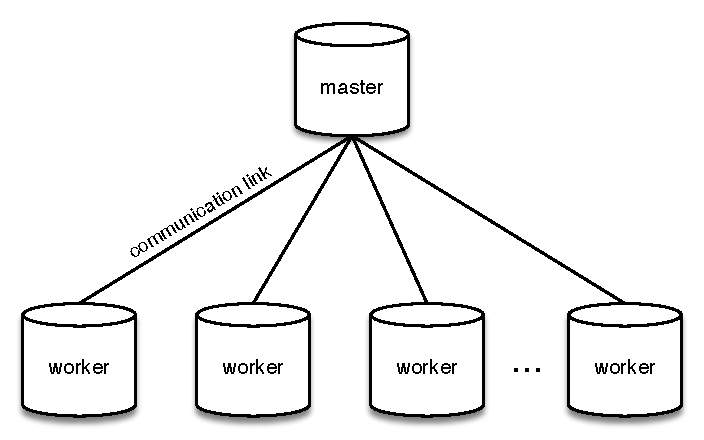
\includegraphics[scale=0.8]{distributed_architecture.pdf}
  \caption{Network architecture employed by the proposed algorithm}
  \label{fig:distributed_architecture}
\end{figure}

\subsection*{Parameters of the algorithm}
The proposed method comprehends four parameters, namely $k$, $\mathsf{Eps}$, $\mathsf{MinPts}$ and $\omega$. The value of parameter $k$ represents the size of the neighborhood over which the SNN similarity measure is going to be computed. The neighborhood of each data point is calculated using a proximity function in the original feature space (e.g. term-space in the case of documents). Then, in the SNN space, the value of $\mathsf{Eps}$ denotes the similarity threshold beyond which two points are considered as close. The similarity in the SNN space corresponds to the number of shared neighbors between two different data points. Additionally, a point is identified as a \textit{core-point} when the number of points close to it in the SNN space surpasses the value of the density parameter $\mathsf{MinPts}$. Finally, the value of the parameter $\omega$ rules the size of the sample set of \textit{core-points} that is going to be transmitted to the master node.

\subsection*{Initial stage}
This stage starts by working over each data partition. 
%Data partition may be obtained by randomly partitioning and distributing the dataset into several worker nodes.
In this primary stage, each worker $n_i$ starts identifying in its partition $\mathcal{D}_i$ the core-points by following the procedure $\mathsf{SnnCorePoints}$ described in algorithm \ref{alg:snncorepointid}. The procedure starts by computing the k-nearest neighbors of each data point in $\mathcal{D}_i$. To deal with high dimensional data, we use in this step the cosine similarity. Note that this function may be replaced with a better one depending on the nature of the data. Then, we calculate the size of the shared neighborhood for every pair of distinct points in $\mathcal{D}_i$, a value that in algorithm \ref{alg:snncorepointid} is indexed by the function named $\textsc{SNN}_k(p,q)$. Then, for each data point in $\mathcal{D}_i$ we calculate its density which corresponds to the number of data points 
whose shared neighborhood is greater than $\mathsf{Eps}$. Finally, the algorithm \ref{alg:snncorepointid} checks the core point condition. Each point is marked as a core point if its density is greater than $\mathsf{MinPts}$. The collection of core points is returned by the algorithm to the cluster labeling process, described in algorithm \ref{alg:coresample}. Note that the similarity function $\textsc{SNN}_k(p,q)$ is also returned. 

\iffalse
\begin{algorithm}[!htbp]
   \DontPrintSemicolon
  \SetKwFunction{snncpts}{SnnCorePoints}
  \SetKwProg{Fn}{Function}{:}{}
  
  \Fn{\snncpts{$\mathcal{D}_i$, $k$, $\mathsf{Eps}$, $\mathsf{MinPts}$}}{
  \ForEach{$p\in\mathcal{D}_i$}{compute $KNN_{k}(p)$\;}
  \ForEach{$p\in \mathcal{D}_i$}{
  	\ForEach{$q\neq p\in \mathcal{D}_i$}{
		$\mathsf{SNN}_{k}(p,q)\leftarrow \left\vert{KNN_{k}(p)\cap KNN_{k}(q)}\right\vert$\; 
    }
    $\mathsf{density}(p)\leftarrow \left\vert{\{q\neq p\in\mathcal{D}_i:\mathsf{SNN}_{k}(p,q)>\mathsf{Eps}\}}\right\vert$\;
    \lIf{$\mathsf{density}(p)>\mathsf{MinPts}$}{Mark $p$ as \textbf{core-point}}
  }
$\mathcal{C}_i\leftarrow$ all points marked as  \textbf{core-point} in $\mathcal{D}_i$\;
\KwRet $\mathcal{C}_i$ , $\mathsf{SNN}_{k}$\;
  }
\caption{Identification of core-points from a data partition $\mathcal{D}_i$}
\label{alg:snncorepointid}
\end{algorithm}

\begin{algorithm}[!htbp]
% \KwData{$\mathcal{D}$ denotes the local subset of the data, $k$, $\mathsf{Eps}$, $\mathsf{MinPts}$, $\omega\in [0,1]$}
% \KwResult{List of representative points per group}
 \DontPrintSemicolon
  \SetKwFunction{sampleld}{SampleLocalData}
  \SetKwProg{Fn}{Function}{:}{}
  
  \Fn{\sampleld{$\mathcal{D}_i$, $k$, $\mathsf{Eps}$, $\mathsf{MinPts}$, $\omega\in [0,1]$}}{
  
  $\mathcal{C},\mathsf{SNN}_k\leftarrow$ \snncpts{$\mathcal{D}_i$, $k$, $\mathsf{Eps}$, $\mathsf{MinPts}$}\;
  
 \ForEach{\bf{core-point} $p\in \mathcal{C}$}{
 	\If{$p$ is not visited}{
    	Assign a new cluster label $l_p$ to $p$\;
	mark $p$ as visited\;
    	\ForEach{Not visited $q\neq p\in\mathcal{C}$}{
        	\If{$\mathsf{SNN}_{k}(p,q)>\mathsf{Eps}$}{
            	Assign label $l_p$ to $q$\;
		mark $q$ as visited\;
            }
    	}
    }    
}
 $N_c\leftarrow$Number of labeled \bf{core-points}\;
 $S\leftarrow\emptyset$\;
 \ForEach{cluster}{
 	$S\leftarrow$ Add $\omega\cdot N_l$ points sampled from group $l$ with weight $\dfrac{1 - ( N_l/N_c ) }{2\cdot N_l}$\;
 }
 \KwRet sampled data $S$\;%en L124 se ejecuta el cludtering sobre los datos centralizados.
 }
\caption{Selection of representative points executed in a node}
 \label{alg:coresample}
\end{algorithm}
\fi


%\subsubsection*{Labeling step}
Then the algorithm continues with a labeling process, which works as follows. Initially, all points are unlabeled. Then, we assign the same cluster label to each core point that belongs to the same connected component, i.e. the collection of points that mutually has at least a $\mathsf{Eps}$ similarity in the SNN space. Accordingly, a cluster is defined as a high density region of data points in the \textit{SNN} space. 

Once all core-points are labeled, a weighted sample from each cluster is drawn. The weight of a data point follows the expression:\[\dfrac{1 - ( N_l/N_c ) }{2\cdot N_l}\] where $N_c$ denotes the number of labeled core-points and $N_l$ the number of points labeled with label $l$. The expression shown above denotes that the sampling weight of a core-point is inverse to its group size as it is depicted in Figure \ref{fig:group_weight}. The aim of this function is to build a sample of core-points able to represent both small and large groups alike without a bias to larger clusters which is a serious problem for clustering algorithms operating under unbalanced data scenarios.
This procedure is described in the last lines of algorithm \ref{alg:coresample}. 

\begin{figure}[!htbp]
\centering
  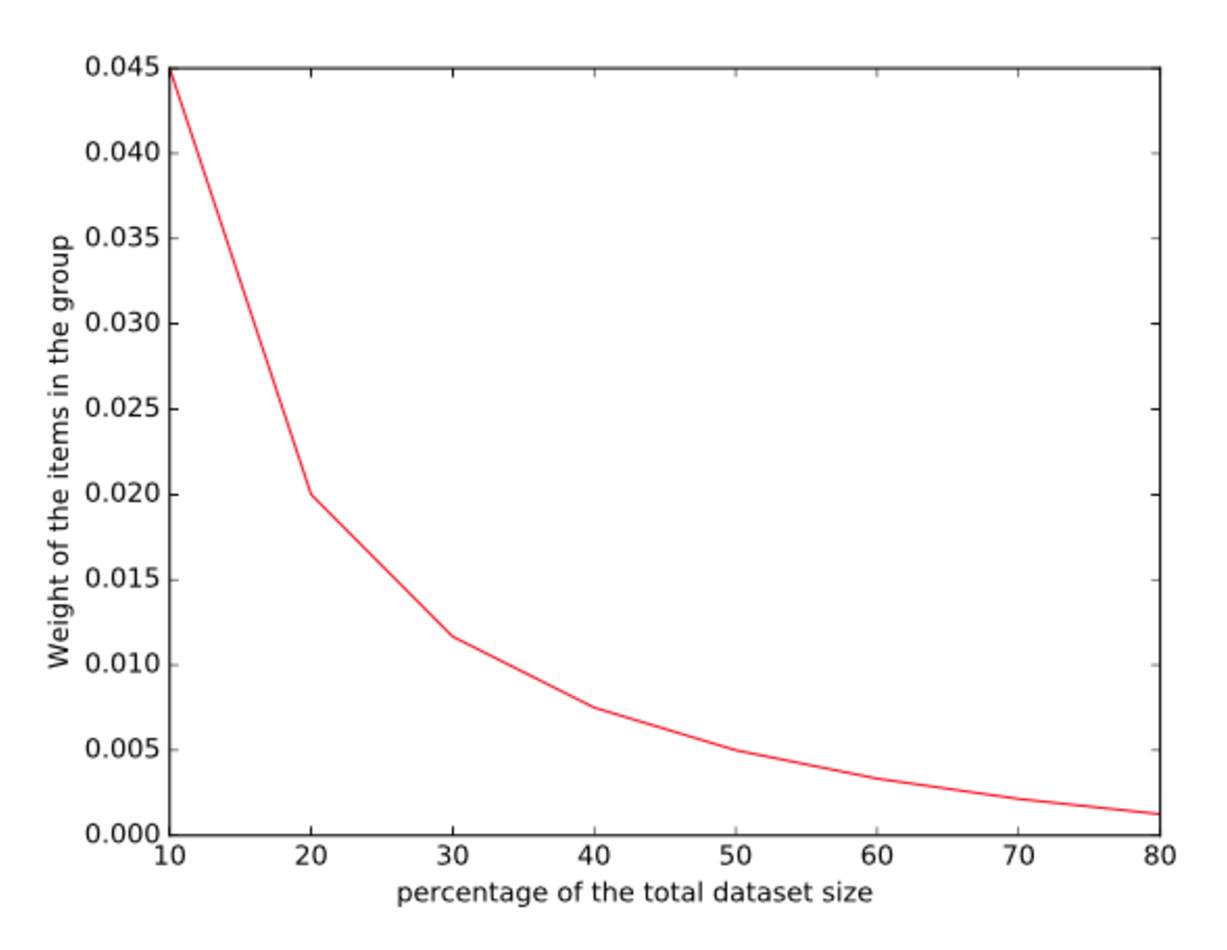
\includegraphics[scale=0.6]{group_weights.pdf}
  \caption{Weight of each item in a group vs the relative size of the group in comparison with the data set size.}
  \label{fig:group_weight}
\end{figure}

%\subsubsection*{Identification of core-points}
% TODO: no se que poner aqui aun!!
\subsection*{Final stage}
This stage starts when all worker nodes transmit their sample of core-points to the master node and then this node joins all these points into a single data set $\mathcal{S}$. 
%As this overall sample contains $\omega[\pct]$ of the dataset, its processing cost is much smaller than the one involved in processing the complete collection. 
Then the procedure $\mathsf{SnnCorePoints}$ is applied over $\mathcal{S}$, obtaining a new core-point set $\mathcal{C}$, and the same labeling step applied in the initial stage in each worker is performed over this set. After this step, for each point $q\in\mathcal{S}$ not chosen for the core-point set $\mathcal{C}$, its nearest neighbor  $p\in\mathcal{C}$ is found. If the SNN similarity between these points is lower than $\mathsf{Eps}$, then $q$ is marked as noise, otherwise label $l_p$ is assigned to $q$.
Finally, the set of labeled points in $\mathcal{S}$ (i.e. discarding the noisy subset) is returned.
A thorough description appears in algorithm \ref{alg:centralproc}.



\begin{algorithm}[!htbp]
 \KwData{$\mathcal{D}$: entire dataset, $\mathcal{W}$: set of workers, $\eta$: sampling percentage, master and workers snn--params}
 
 \KwResult{Partition of the overall dataset}
 \DontPrintSemicolon
 \SetKwFunction{stageonew}{stage1\_worker}
 \SetKwFunction{stagetwow}{stage2\_worker}
  \SetKwFunction{master}{master\_procedure}
  \SetKwProg{Fn}{Function}{:}{}
  \Fn{\master{$\mathcal{D}$, $\mathcal{W}$, $\eta$, $\mathsf{Eps}_{m}$, $\mathsf{MinPts}_{m}$, $\mathsf{Eps}_{w}$, $\mathsf{MinPts}_{w}$}}{
  %$Q\subset \mathcal{P}(\mathcal{D})\leftarrow random\_sample(\mathcal{D},|\mathcal{W}|)$\;
  $Q\subset \mathcal{P}(\mathcal{D})\leftarrow Q_{w_{1}}\cup Q_{w_{2}}\ldots Q_{w_{|\mathcal{W}|}}$\SetNoFillComment{ uniformly drawn!}\;
  $C\leftarrow \{\}$\;
  $S\leftarrow \{\}$\;
   \ForEach{$w \in \mathcal{W}$}{
   	$C_{w},S_{w}\leftarrow\stageonew(Q_{w},\eta, \mathsf{Eps}_{w}, \mathsf{MinPts}_{w})$\;
	$C\leftarrow C\cup C_{w}$\;
	$S\leftarrow S\cup S_{w}$\;
   }
  $\mathbf{A}\leftarrow$adjacency\_matrix$(S\cup C)$\;
  
  \SetSideCommentLeft{\#$C'\subset \mathcal{\{S\cup C\}},L'\subset \mathcal{P}(\mathcal{\{S\cup C\}}),\mathcal{N}'\subset \mathcal{\{S\cup C\}}$}\;
  $C',L',\mathcal{N}'\leftarrow$centralized\_snn$(\mathbf{A},\mathsf{Eps}_{m},\mathsf{MinPts}_{m})$\;
  $L\leftarrow \{\}$\;
  \ForEach{$P \in L'$}{
  	$L\leftarrow L\cup \{\{x\in P , x \in C' \}\}$\;
  }
  \ForEach{$w \in \mathcal{W}$}{
  	$L_{w}\leftarrow \stagetwow(Q_{w}, C',L)$\;
	\ForEach{$p \in L_{w}$}{
		$g\leftarrow \{q\in L \ s.t.\ |p\cap q|>0\}$\;
		$L\leftarrow \{L\setminus g\}\cup  \{g\cup p\}$\;
	}
  }
   \KwRet $L$\;
}
\caption{Procedure executed by the master node}
 \label{alg:centralproc}
\end{algorithm}


\begin{algorithm}[!htbp]
% \KwData{$\mathcal{D}$ denotes the local subset of the data, $k$, $\mathsf{Eps}$, $\mathsf{MinPts}$, $\omega\in [0,1]$}
 \KwResult{Set of core-points and a set with sample data from each group}
 \DontPrintSemicolon
  %\SetKwFunction{stageonew}{stage1\_worker}
  \SetKwProg{Fn}{Function}{:}{}
  \Fn{\stageonew{$\mathcal{X}$, $\eta$, $\mathsf{Eps}$, $\mathsf{MinPts}$}}{
  $\mathbf{A}\leftarrow$adjacency\_matrix$(\mathcal{X})$\;
  \SetSideCommentLeft{\#$C_\mathcal{X}\subset \mathcal{X},L_\mathcal{X}\subset \mathcal{P}(\mathcal{X}),\mathcal{N}_\mathcal{X}\subset \mathcal{X}$}\;
  $C_\mathcal{X},L_\mathcal{X},\mathcal{N}_\mathcal{X}\leftarrow$centralized\_snn$(\mathbf{A},\mathsf{Eps},\mathsf{MinPts})$\;
  $S\leftarrow\{\}$\;
   \ForEach{$L_{i} \in L_\mathcal{X}$}{
   	$S_{i}\leftarrow$get\_random\_sample$(L_{i},\eta*|L_{i}|)$\;
	$S\leftarrow S\cup \{S_{i}\}$
   }
   \KwRet $C_\mathcal{X}, S$\;
}
\caption{Stage 1 -- worker procedure}
 \label{alg:stage1w}
\end{algorithm}

\begin{algorithm}[!htbp]
% \KwData{$\mathcal{D}$ denotes the local subset of the data, $k$, $\mathsf{Eps}$, $\mathsf{MinPts}$, $\omega\in [0,1]$}
 \KwResult{Partition of the dataset given to the worker}
 \DontPrintSemicolon
  %\SetKwFunction{stagetwow}{stage2\_worker}
  \SetKwProg{Fn}{Function}{:}{}
  \Fn{\stagetwow{$\mathcal{X}$, $C$, $L_\mathcal{C}$}}{
  $L\subset \mathcal{P}(\mathcal{X})\leftarrow \{\}$\;
   \ForEach{$x \in \mathcal{X} \setminus C$}{
   	\SetSideCommentLeft{\#label $x$ with the label of its nearest corepoint}\;
	$c\leftarrow \argmax_{q\in C}sim(x,q)$\;
	$g\leftarrow r\in L | c\in r$\;
	$L\leftarrow \{L\setminus g\}\cup \{g\cup \{x\}\}$\;
   }
   \KwRet $L$\;
}
\caption{Stage 2 -- worker procedure}
 \label{alg:stage2w}
\end{algorithm}

\subsection*{Cost of the algorithm}

Assuming that $D$ has $n$ data points and the system works over $P$ nodes, 
the cost of the SNN space construction per node is $\Theta\left(\dfrac{n^2}{P^2}\right)$. 
The cost of the labeling process per node is linearly upper bounded by the partition size $\mathcal{O}(\dfrac{n}{P})$ (the worst case happens when the entire partition is marked as core point). 
The cost of data transmission per node is ruled by $\omega$ and is upper bounded by the partition size $\mathcal{O}(\omega \cdot \dfrac{n}{P})$. In the master node, the size of the centralized core sample $S$ is upper bounded by $\mathcal{O}(\omega \cdot n)$. Then, the construction of the SNN space over $S$ costs $\Theta\left( \omega^2 \cdot n^2 \right)$. The cost of the labeling process is upper bounded by the size of $S$, then its cost is $\mathcal{O}(\omega \cdot n)$. 

As the costs are governed by the quadratic costs involved in SNN construction, the total cost of D-SNN is ruled by $\Theta\left( \left( \dfrac{1}{P^2} + \omega^2 \right) \cdot n^2 \right)$. The factor $\dfrac{1}{P^2} + \omega^2$ represents the fraction of C-SNN that D-SNN is able to reduce.

\subsection*{Illustrative example}

We provide an illustrative example by applying D-SNN over the synthetic data set shown in Figure \ref{fig:toy_original} which was proposed by Guha \textit{et al.} \cite{GRS98} when the algorithm CURE was introduced. As Figure \ref{fig:toy_original} shows, the data set contains five clusters, depicted with different colors, and noise points (app. 2,000 points over a data set of 70,000 2D data points). The algorithm was executed over 8 disjoint data partitions created using uniform sampling at random. The SNN space was created using Euclidean neighborhoods of 90 data points. We used $\mathsf{MinPts} = 30$ and $\omega = 0.3$. Results for $\mathsf{Eps} = 50, 60$ are shown in Figures \ref{fig:toy_dsnn1} and \ref{fig:toy_dsnn2}, respectively.  

\begin{figure}[!htbp]
\centering
  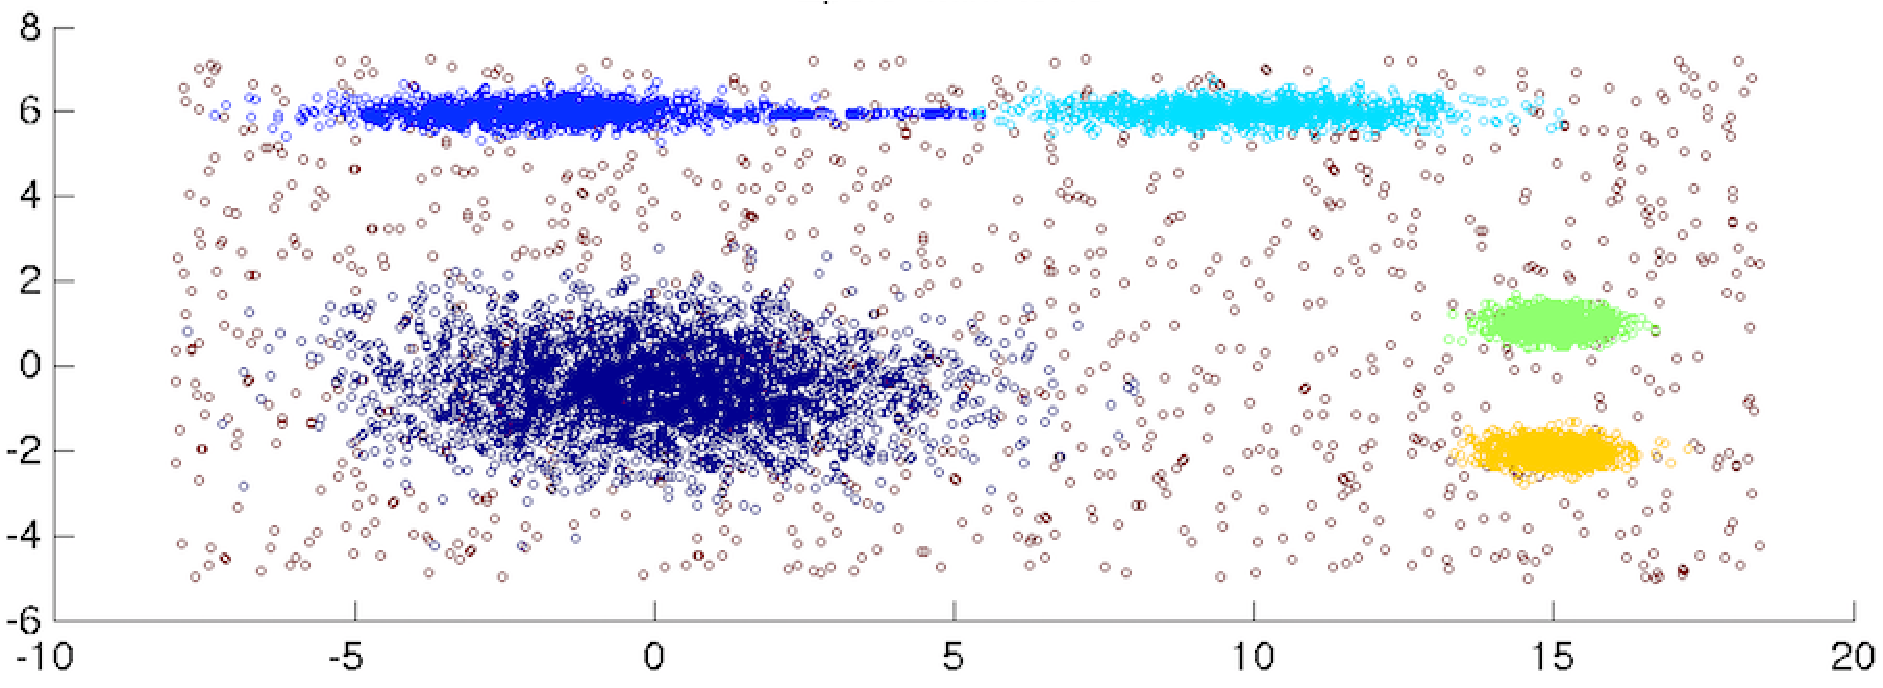
\includegraphics[scale=0.47]{toy_example_original.pdf}
  \caption{Simulated data used in our example.}
  \label{fig:toy_original}
\end{figure}

\begin{figure}[!htbp]
\centering
  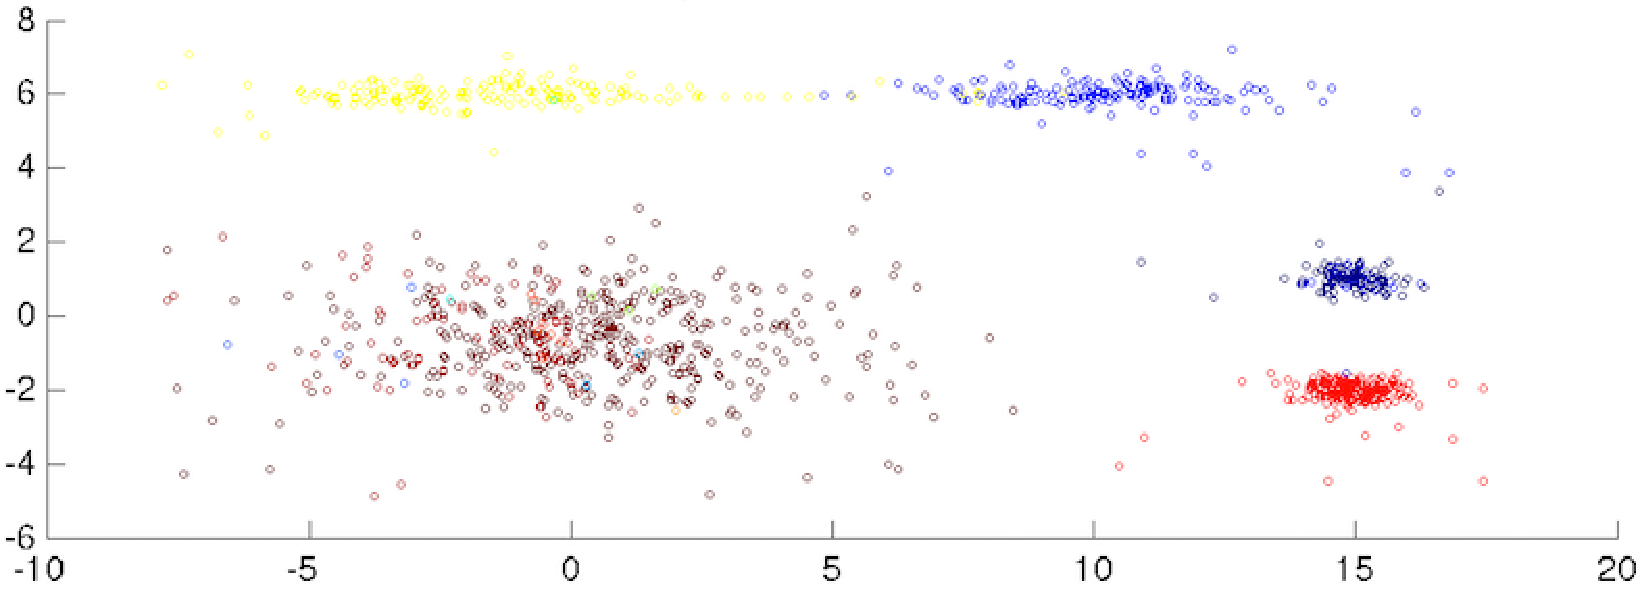
\includegraphics[scale=0.54]{toy_example_after_Dsnn_2.pdf}
  \caption{Data after D-SNN clustering with $\mathsf{Eps}=50$.}
  \label{fig:toy_dsnn1}
\end{figure}

\begin{figure}[!htbp]
\centering
  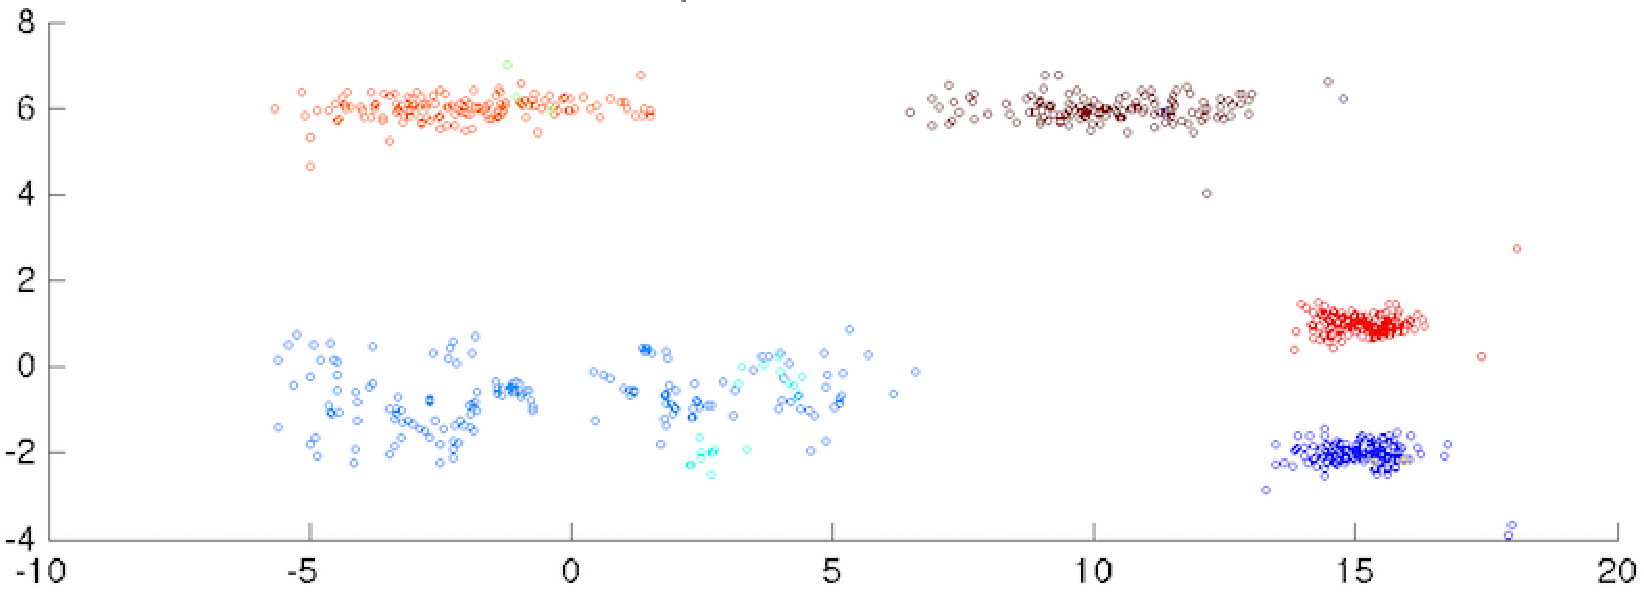
\includegraphics[scale=0.54]{toy_example_after_Dsnn_1.pdf}
  \caption{Data after D-SNN clustering with $\mathsf{Eps}=60$.}
  \label{fig:toy_dsnn2}
\end{figure}

As figures \ref{fig:toy_dsnn1} and \ref{fig:toy_dsnn2} show, the effectiveness of the distributed algorithm and its robustness to noise is illustrated. 
By contrasting Figure \ref{fig:toy_original} against \ref{fig:toy_dsnn1} and \ref{fig:toy_dsnn2}, it is noticed that the noise layer was successfully removed by the clustering algorithm in both cases. Note that the $\mathsf{Eps}$ value had an impact in the sensitivity of the algorithm to detect noise points, i.e. a high value for this parameter was accompanied by an increasing rate of points marked as noise as it is specially noticed in the bridge of points that connects the two ellipsoids in Figure \ref{fig:toy_original}. We will study the sensitivity of our algorithm to parameters in the next section. 

\section{Methodology and Experimental results}
\label{sec:exps}

In this section, we assess the performance of D-SNN on five data sets comparing its effectiveness against C-SNN \cite{ESK03}. 
In addition we include other two methods in the evaluation: Firstly, a SNN-graph bisection method successfully employed in text clustering tasks \cite{ZK02}. Secondly, a parallel version of Kmeans++ proposed by \cite{BMVKV12} and successfully implemented into the Spark Framework. In this section, the former algorithm is denoted as \textit{Graph Clust} and the latter is denoted as \textit{Kmeans$||$}.

Each data set was partitioned into 4 disjoint partitions produced by a uniform sampling process at random. 
Then, each partition was distributed onto the different nodes in which the initial stage procedure was performed. 
Then, the results obtained after performing the final stage procedure in the master node were accounted.
% se podrian presentar brevemente los métodos con que se comparará
% se podria introducir aqui los hallazgos que encontramos luego de los experimentos.

\subsection*{Data sets}

The experiments were performed over 5 data sets containing documents represented as vectors in high dimensional term spaces. 
We use the well known text data set 20-Newsgroups (M5 partition), a document collection that contains almost 5000 news coming from different subjects, namely computers, motorcycles, baseball, science and politics. The remaining four document sets were extracted from the Tipster collection~\footnote{https://tac.nist.gov/data/data$\_$desc.html}. In specific, we include in our evaluation \textit{DOE}, a data set which contains short abstracts of the Department of Energy, \textit{FR} which contains reports of actions taken by U.S. government agencies, \textit{SJMN}, a collection of news published by the San Jose Mercury news, and \textit{ZF}, a collection of news about computers published by Ziff-Davis Publishing Co.

In table \ref{table:datasets}, we summarize the number of documents, the size of the vocabulary, the number of classes and the percentage of non zero values (a measure of the sparsity of the collection) per data set. Note that all these collections are quite sparse and also their document vectors are spanned onto high dimensional term spaces with tens of thousands of features. 

\begin{table}[htbp]
\centering
\noindent\adjustbox{max width=\textwidth}{%
\begin{tabular}{llrrrc}
    \hline
    Dataset & Description &instances & $|\set{V}|$ & classes & $\pct$NNZ\\ \hline
\textit{20NG} & 20-newsgroup data, m5 partition. & $4743 $ & $41223$ & $5$   & $0.167\pct$ \\     
\textit{DOE} &  Department of Energy Abstracts& $1664$ & $15755 $ & $14$     & $0.365\pct$ \\ 
\textit{FR} & Federal Register notes& $926 $ & $50427 $ & $14$               & $1.104\pct$ \\ 
\textit{SJMN} & San Jose Mercury News & $908 $ & $23616$ & $16$              & $0.738\pct$ \\ 
\textit{ZF} & Computer select disks by Ziff-Davis & $3263 $ & $58398 $ & $25$& $0.360\pct$ \\ \hline % end of tipster.
\end{tabular}}
\caption{Data sets employed.}
\label{table:datasets}
\end{table}

\subsubsection*{Document processing}

To obtain a representative set of terms for each collection, i.e. its index terms, the documents were processed following the steps indicated in Figure \ref{fig:text_processing}. This figure shows standard text processing steps commonly used in information retrieval and text mining tasks. Firstly, as documents within the Tipster collections come in SGML format, their content were extracted. Then, spacing and punctuation marks were removed in order to keep only the candidate terms of the vocabulary. After this step, the set of candidate terms was filtered using an English stop-word set, which aids to remove meaningless words (e.g. \textit{the}, \textit{of}, \textit{by}). 

None other process was applied to the documents in this work (e.g. stemming) in order to keep the text content as similar as possible to the original source and specially to allow subsequent generalizations of the performance results of the proposal without any tie to a specific data set. 
Finally, the selected terms within each collection were sorted and then the vocabulary was obtained (the vocabulary size reported in table \ref{table:datasets} corresponds to the vocabulary obtained after document processing).

\begin{figure}[!htbp]
\centering
  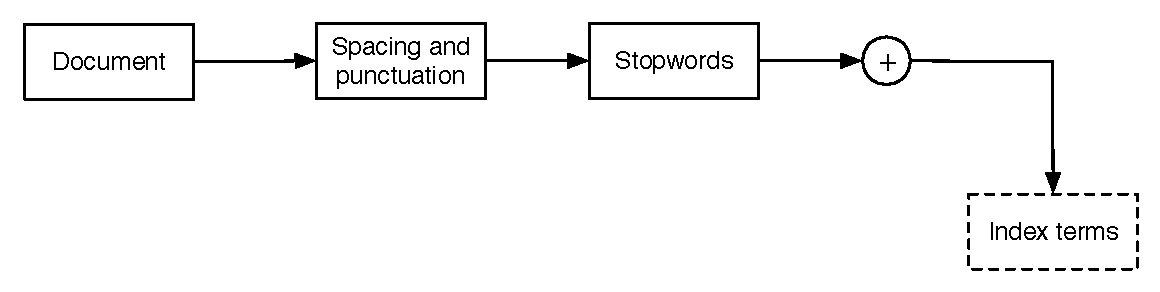
\includegraphics[scale=0.7]
  {text_processing_steps.pdf}
  \caption{Text processing steps performed in each collection.}
  \label{fig:text_processing}
\end{figure}

After the vocabulary of each collection was built, the number of occurrences of its terms in each document was computed and used to build the vector representation of each document. 
Let $f_{i,j}$ be the number of occurrences of a term $i$ of the vocabulary $\mathcal{V}$ in the document $j$ of the collection.
Let $n_{i}$ be the number of documents of the collections that contain the term $i$.
The weight of term $i$ within a document $j$ is quantified by the expression:

\[w_{i,j}=\frac{f_{i,j}}{ \operatorname*{max}_{t\in \mathcal{V}}f_{t,j} }\cdot\log\frac{n}{n_{i}}\] 

which corresponds to the Tf-Idf weight of the term $i$ for $j$.

We use the cosine proximity to measure the similarity between each pair of document in each data set. 
To understand differences and similarities across data sets, we plot their similarity matrices.
The documents were sorted consecutively by the group label. 
In each matrix, we plotted similarities using gray scale. 
Darker spots denote high similarity values. 
These matrices are shown in Figure \ref{fig:sim_matrices}. 

\begin{figure}[!htbp]
    \centering
    \begin{subfigure}[b]{0.33\textwidth}
        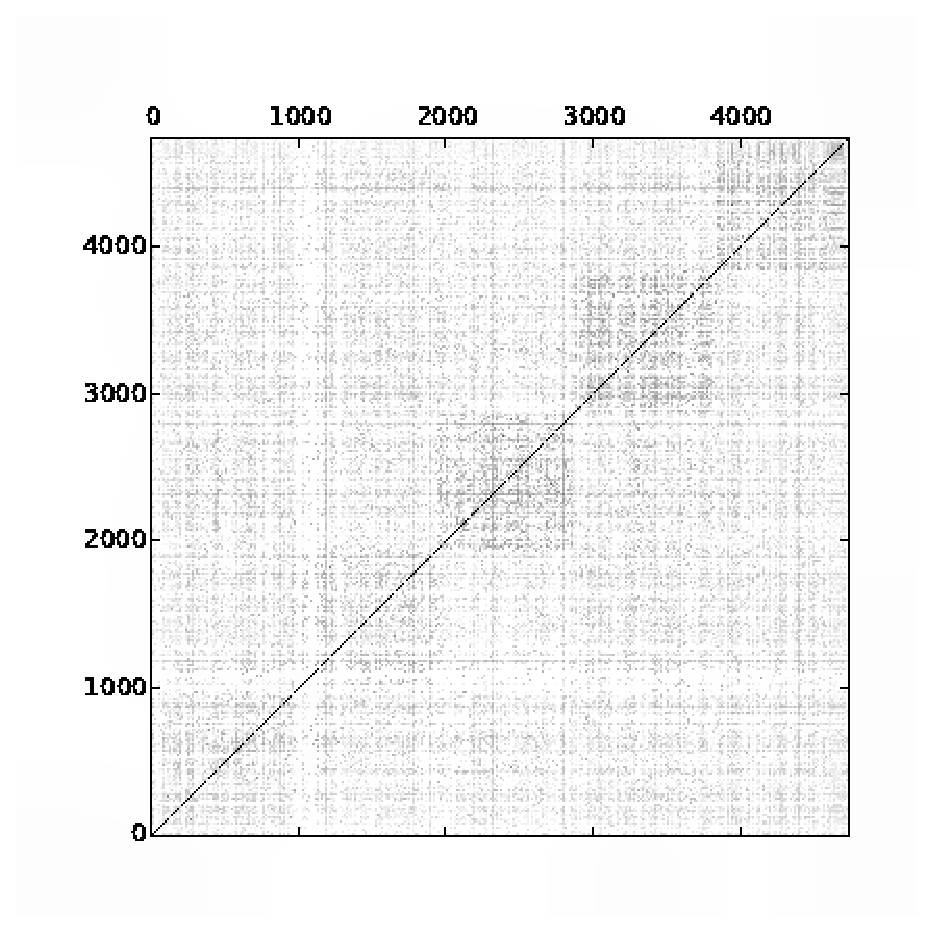
\includegraphics[width=\textwidth]{./similarities/20NG-simcos}
        \caption{The 20NG collection.}
        \label{fig:20ng_sim}
    \end{subfigure}
    \begin{subfigure}[b]{0.33\textwidth}
        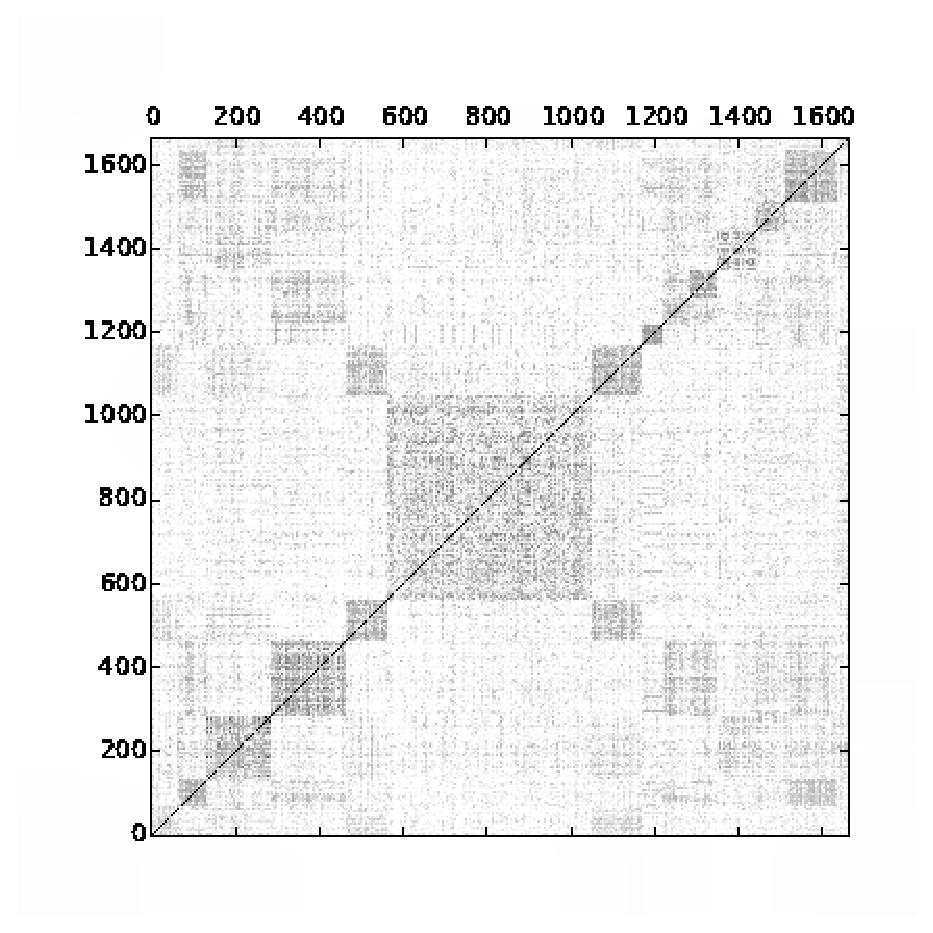
\includegraphics[width=\textwidth]{./similarities/DOE-simcos}
        \caption{The DOE collection.}
        \label{fig:doe_sim}
    \end{subfigure}
    \begin{subfigure}[b]{0.33\textwidth}
        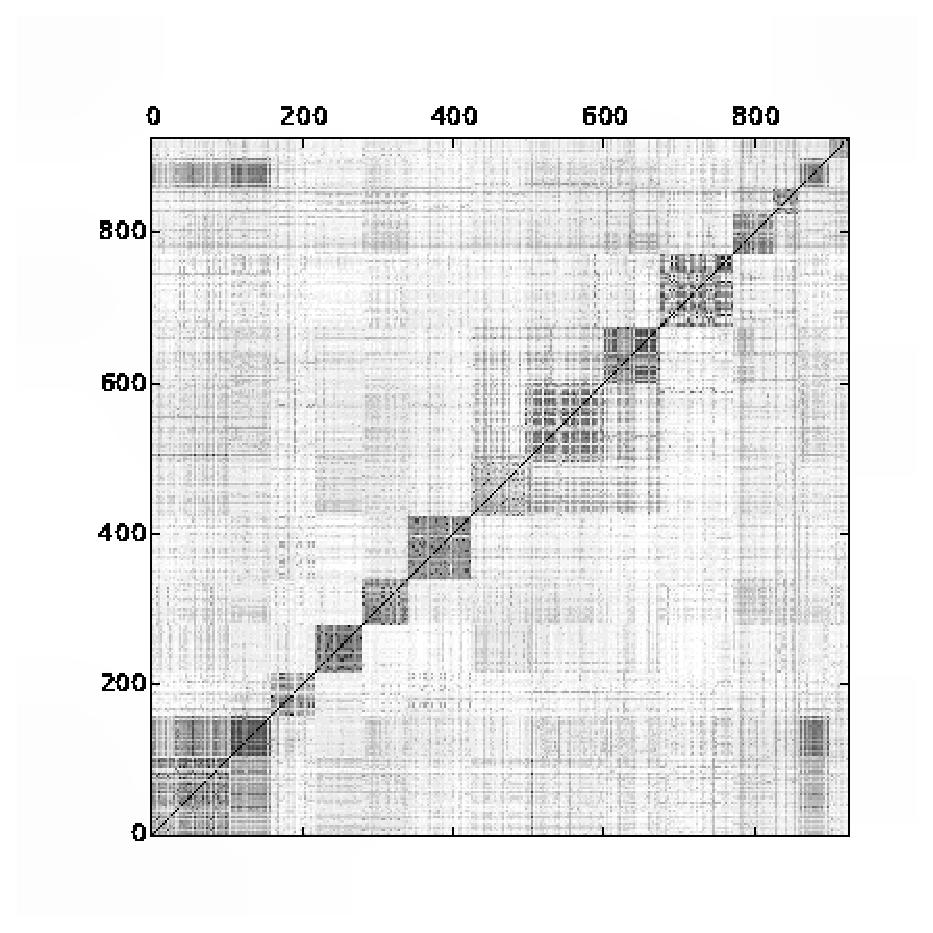
\includegraphics[width=\textwidth]{./similarities/FR-simcos}
        \caption{The FR collection.}
        \label{fig:fr_sim}
    \end{subfigure}
    \begin{subfigure}[b]{0.33\textwidth}
        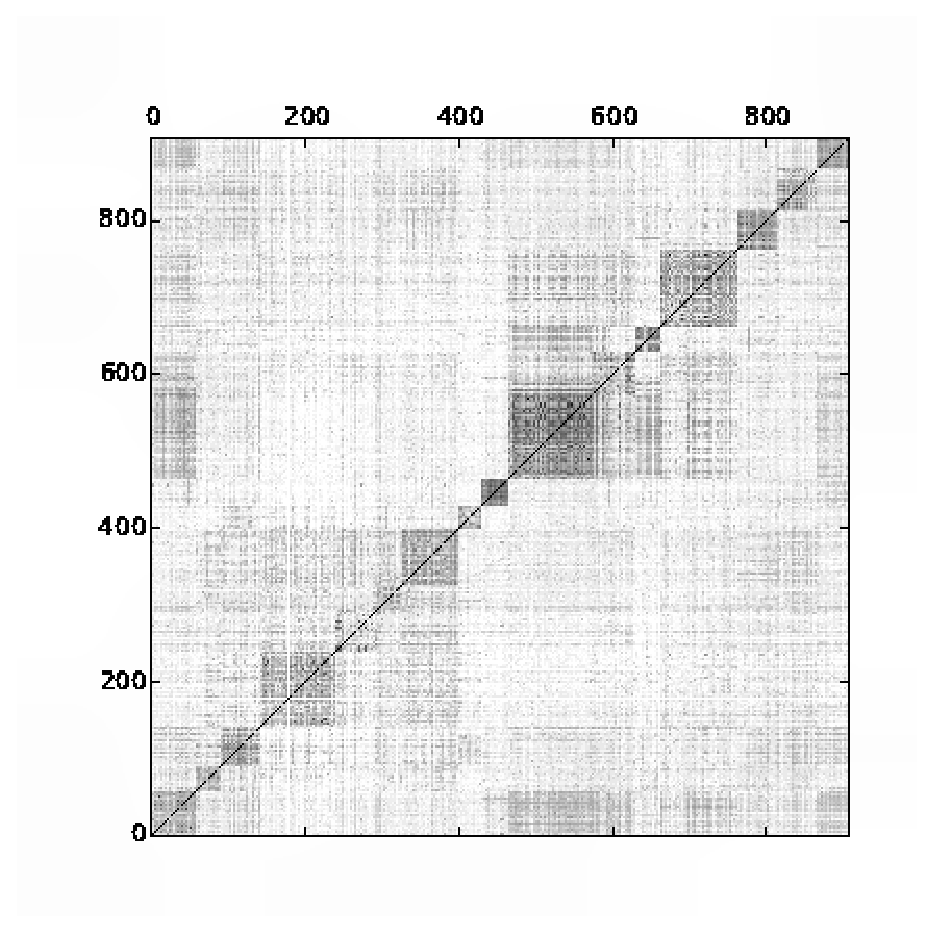
\includegraphics[width=\textwidth]{./similarities/SJMN-simcos}
        \caption{The SJMN collection.}
        \label{fig:sjmn_sim}
    \end{subfigure}
    \begin{subfigure}[b]{0.33\textwidth}
        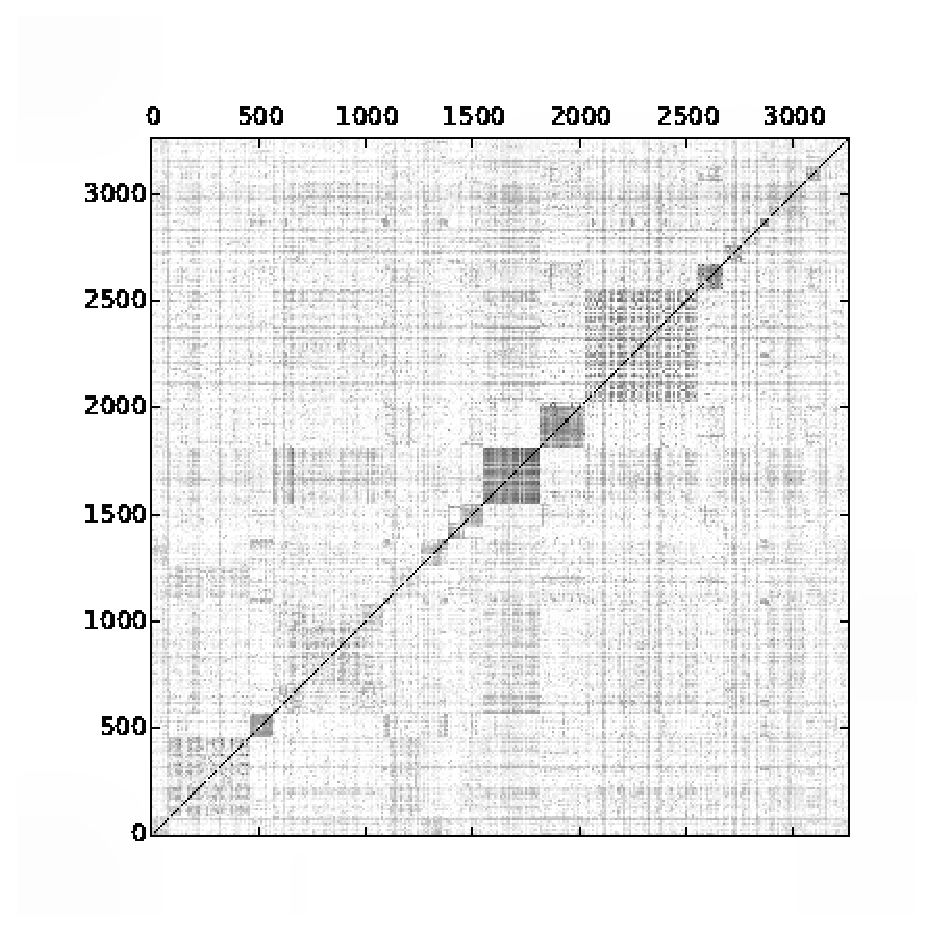
\includegraphics[width=\textwidth]{./similarities/ZF-simcos}
        \caption{The ZF collection.}
        \label{fig:zf_sim}
    \end{subfigure}    
    \caption{Pairwise cosine-similarity matrices}\label{fig:sim_matrices}
\end{figure}

The matrices plotted in Figure \ref{fig:sim_matrices} show darker rectangular patches along the diagonal line, showing the presence of clusters. 
In addition, 20NG and ZF show pairwise similarities not much higher than the ones outside the clusters, suggesting that the data points in these data sets are very sparse. 
In the case of the DOE collection, some spots outside the diagonal appear suggesting the existence of cluster overlapping.
Finally, the SJMN collection shows small squares embedded into big squares along the diagonal suggesting the existence of nested clusters.

\subsection*{Clustering quality measures}

In this work, only external validation measures were employed, namely \textbf{Adjusted-Mutual-Information}, \textbf{Homogeneity}, \textbf{Completeness} and  \textbf{V-Measure}. 

The \textbf{Adjusted-Mutual-Information} measure was proposed in \cite{VEB10} and evaluates how much information of the true labeling is represented into the resulting clustering. The \textbf{Homogeneity} measures the extent in which the clusters contain only data points which are members of a single class. The \textbf{Completeness} accounts for the extent in which all the data points that are members of a given class are elements of the same cluster. The \textbf{V-Measure} corresponds to the harmonic mean between \textbf{Homogeneity} and \textbf{Completeness}. These scores, with the exception of the Adjusted-Rand-Index which is within $[-1,1]$, have positive values within $[0,1]$. For all of these measures, larger values denote a better clustering quality.

%\textbf{Entropy}, measures the extent in which all data from one class are spread into several groups and 
%\textbf{Purity} measures the extent that a cluster contains only one class of data. 
%\textbf{Adjusted-Rand-Index} measures the matching between the true labels and the ones produced by the algorithm under study by counting the proportion of point-pairs whose relationship is the same in both labelings. 

\subsection*{Grid search of parameters}

To report the best performance found for each algorithm, we conducted a grid search for $K$, $\mathsf{Eps}$ and $\mathsf{MinPts}$. The results were evaluated in terms of \textbf{V-Measure}. We used the same grid for C-SNN and D-SNN.
The grid used consists of $432$ configurations with $K$ in $\{15, 30, 50, 70, 90, 110\}$, $\mathsf{Eps}$ in $\{3, 5, 8, 10, 15, 20, 25, 30, 35, 40, 45, 50\}$ and $\mathsf{MinPts}$ in $\{5, 10, 15, 20, 25, 30\}$. For the \textit{Graph Clust} algorithm the same values for $K$ were tested but no difference in the performance was detected. Additionally, since the \textit{Graph Clust} and \textit{Kmeans$||$} algorithms require the number of groups as a parameter, it was correspondingly set to the known number of classes of each dataset.
We show the best parameters for C-SNN and D-SNN in Tables \ref{table:centralizedsnn_params} and \ref{table:distributedsnn_params}, respectively.

\begin{table}[!htbp]
\centering
\begin{tabular}{l|crr}
\textbf{Dataset} & \textbf{K} & \textbf{Eps} & \textbf{MinPts} \\ \hline
20NG    & 110& 25 & 30 \\
DOE     &  70& 25 & 30 \\
FR      &  50& 25 & 20  \\
SJMN    &  50& 20 & 30 \\
ZF      &  90& 40 & 25 \\ \hline
\end{tabular}
\caption{Parameters of the C-SNN clustering algorithm selected after the grid search of parameters.}
\label{table:centralizedsnn_params}
\end{table}

\begin{table}[!htbp]
\centering
\begin{tabular}{l|crr}
\textbf{Dataset} & \textbf{K} & \textbf{Eps} & \textbf{MinPts} \\ \hline
20NG    & 30& 8 & 25 \\
DOE     & 30& 10& 20 \\
FR      & 30& 10& 5  \\
SJMN    & 30& 10& 10 \\
ZF      & 30& 10& 15 \\ \hline
\end{tabular}
\caption{Parameters of the D-SNN clustering algorithm selected after the grid search of parameters.}
\label{table:distributedsnn_params}
\end{table}

In the case of D-SNN, we run our experiments using $w = 0.3$ over 4 partitions. 

\subsection*{Results} % TODO: Comentar algo respecto de los resultados y los parámetros
\iffalse
The  evaluation of the algorithms was made in terms of measuring their capability of 
dealing with low contrast between intra-class and extern pairwise similarities (low discrimination power of the similarity measure), 
the presence of classes with unequal sizes and 
the existence of hierarchical relations between the classes.
\fi

The results of our experiments are shown in Table \ref{table:results}. 
Bold fonts indicate the best result for each configuration. 

\begin{table}[!htbp]
\centering
\begin{tabular}{cl|clll}
%ARI(3) AMI(4) NMI(5) HOM(6) COM(7) VMea(8)
&\textbf{Dataset} & \textbf{AMI}  & \textbf{HOM} & \textbf{COM} & \textbf{VM} \\ \hline
%CLUTO
\parbox[t]{2mm}{\multirow{5}{*}{\rotatebox[origin=c]{90}{Graph Clust}}}&20NG   &  0.6421          &  0.6619          &  0.6425          & 0.6521  \\
&DOE    &  \textbf{0.7030} &  0.7095          &  \textbf{0.7461} & 0.7273  \\
&FR     &  0.7266          &  0.7375          &  0.7452          & 0.7413  \\
&SJMN   &  0.7367          &  0.7505          &  0.7657          & 0.7580  \\
&ZF     &  0.5444          &  0.5593          &  0.6015          & 0.5796  \\ \hline
% CENTRALIZED
\parbox[t]{2mm}{\multirow{5}{*}{\rotatebox[origin=c]{90}{C-SNN}}} &20NG   &  0.3953          &  0.3990          &  0.4793          & 0.4355\\
&DOE    &  0.6370          &  0.6476          &  0.6711          & 0.6591\\
&FR     &  \textbf{0.7834} &  0.7969          &  0.7919          & 0.7944\\
&SJMN   &  0.6820          &  0.7732          &  0.6960          & 0.7326\\
&ZF     & 0.5084           &  0.5750          &  0.5238          & 0.5482\\ \hline
%SPARK KMEANS||(Scalable K-Means++, Bahmani et al. 2012)
\parbox[t]{2mm}{\multirow{5}{*}{\rotatebox[origin=c]{90}{\textit{Kmeans$||$}}}} 
&20NG   & 0.4696  &  0.4702 & 0.5607  & 0.5115  \\
&DOE    & 0.1255  &  0.1344 & 0.6767  & 0.2242  \\
&FR     & 0.3236  &  0.3426 & 0.7062  & 0.4614  \\
&SJMN   & 0.2299  &  0.2518 & 0.6767  & 0.3670  \\
&ZF     & 0.0536  &  0.0648 & 0.6072  & 0.1171  \\ \hline
%DISTRIB
\parbox[t]{2mm}{\multirow{5}{*}{\rotatebox[origin=c]{90}{D-SNN}}} &20NG   & \textbf{0.8218}  &  \textbf{0.8262} & \textbf{0.9167}  & \textbf{0.8691}  \\
&DOE    & 0.7029           &  \textbf{0.8794} & 0.7227           & \textbf{0.7934}  \\
&FR     & 0.7546           &  \textbf{0.8947} & \textbf{0.7784}  & \textbf{0.8325}  \\
&SJMN   & \textbf{0.7836}  &  \textbf{0.8052} & \textbf{0.8040}  & \textbf{0.8046}  \\
&ZF     & \textbf{0.7701}  &  \textbf{0.9882} & \textbf{0.7877}  & \textbf{0.8766}  \\ \hline
\end{tabular}
\caption{Performance attained by the graph clustering algorithm, C-SNN algorithm and D-SNN over the text collections. The best values for each measure in each dataset appear in bold fonts.}
\label{table:results}
\end{table}

\noindent Table \ref{table:results} shows that D-SNN obtains the best performance in almost all the experiments, showing that our algorithm is able to improve clustering quality by conducting density sampling over disjoint partitions. These results are due to the robustness of D-SNN to the presence of noise points. In addition, as density sampling is conducted over disjoint partitions, the robustness of the algorithm is increased, limiting the influence of noise points on clustering. The last fact explains why D-SNN outperforms C-SNN.    

%In most cases D-SNN achieved better scores., nevertheless it is important to mention that a potential improvement is possible for the graph clustering algorithm by applying a better tuning strategy.

As Figures \ref{fig:20ng_sim} and \ref{fig:zf_sim} suggest, 20NG and ZF exhibit a low discrimination power of the underlying similarity measure in the vector term space spanned by the document vectors in each collection. Table \ref{table:results} shows that this phenomenon affects both centralized methods, especially C-SNN in 20NG, by hindering their capability of identifying homogeneous clusters. This is also shown by the lower values of the \textbf{AMI} score attained.

As Figure \ref{fig:doe_sim} shows, DOE is an unbalanced data set, fact that can be evidenced observing the uneven patch sizes along the diagonal in its similarity matrix. 
Table \ref{table:results} shows that D-SNN works well under this scenario. 
This suggests that the shared near neighbor approach helps to address this obstacle.

Figures \ref{fig:fr_sim} and \ref{fig:sjmn_sim} show embedded square patches along the diagonal which suggests a hierarchical structure of the underlying classes. 
Table \ref{table:results} shows that D-SNN works well under this scenario, and accordingly the impact on the performance of nested clusters is successfully drawn by D-SNN.

In summary, our experiments show that the core-point extraction procedure together with the sampling strategy followed to transmit the representatives to the central node enable a much clearer discrimination of each group. Regarding the \textit{Kmeans$||$} algorithm implemented within the Spark framework, it attained poor performance scores over all datasets. This is an expected behavior because of the high dimensional nature of text data and also because the asymmetric sizes of the classes. Finally, it is important to stress that Spark \textit{Kmeans$||$} currently corresponds to one of the most successful implementations of a distributed clustering algorithm in terms of scalability.
%The surrounding patches generally have a lighter gray level in comparison to the inner patches, denoting then that similarities between pairs of documents with different labels are lower than the ones of the pairs having the same label. Nevertheless, this is a common phenomenon in text collections and often hinders the clustering task to prototype-based methods such as K-Means?

%HOM : class distribution within each cluster should be skewed to a single class. (Incluye solamente los puntos de la clase en el cluster)
%COM : the distribution of cluster assignments within each class should be completely skewed to a single cluster. (Incluye todos los puntos de la clase)

% variabilidad de los centralizados en sus desempeños
% costos computacionales debido a al computo secuencial del algorutmo y calculo de matrices de similitud

%\subsection*{Analysis of the results}
 
% dealing with low contrast between intra-class and extern pairwise similarities (low discrimination power of the similarity measure), 
% the presence of classes with unequal sizes and 
% the existence of hierarchical relations between the classes
\iffalse
In summary, the performances achieved by the three algorithms over data sets presenting unequal group sizes and the existence of hierarchical relations between groups are comparable. This is an expected behavior of the shared-nearest-neighbor approach over high dimensional data. %Nevertheless, results interesting that the distributed proposal maintains this capability. 
Results interesting to notice that the performance achieved by the proposal over text collections presenting low contrast between intra-class and extern pairwise similarities is considerably higher than the other two methods under comparison.
\fi
\vspace{-4 mm}
\subsection*{An heuristic for parameter tuning}

In the previous section we showed that D-SNN outperforms C-SNN in almost all the experiments. 
However, the comparison was done using the best values found for the parameters using a grid search. 
The performance of each parameter assignment was evaluated in terms of \textbf{V-Measure}, a performance measure that uses actual labels to measure cluster quality. In an unsupervised learning scenario, D-SNN will work with unlabeled data. Accordingly, in this section we discuss how to tune the parameters of D-SNN on unlabeled data. In order to do this, we present an effective heuristic to tune $\mathsf{Eps}$ and $\mathsf{MinPts}$. 

The heuristic is based on the sorted k-sim graph used by Ester \textit{et al.} \cite{E96} in DBSCAN. The k-sim graph corresponds to the graph of similarities of each point to its k-nearest neighbor. The sorted k-sim graph is the k-sim graph with similarities sorted in decreasing order. As was pointed out by Ester \textit{et al.}, if we use k = $\mathsf{MinPts}$, the sorted k-sim graph shows an inflection point. They selected $\mathsf{Eps}$ from the sorted k-sim graph, value which corresponds to the knee of the curve. 
However, they did not provide a way to determine the value of $\mathsf{MinPts}$. 

Our heuristic comes from the observation of sorted k-sim graphs. 
Note that, in addition to $\mathsf{Eps}$ and $\mathsf{MinPts}$, C-SNN and D-SNN has an additional parameter named $k$, which determines the size of the neighborhood where the SNN space is created. 
We calculate sorted k-sim graphs for different values of $k$. 
Note that $k$ corresponds to the parameter used in the SNN space for similarity calculation, and k is the parameter of the sorted k-sim graph, then $k$ and k are different. 

\begin{figure}[!htbp]
    \centering
    \begin{subfigure}[b]{0.37\textwidth}
        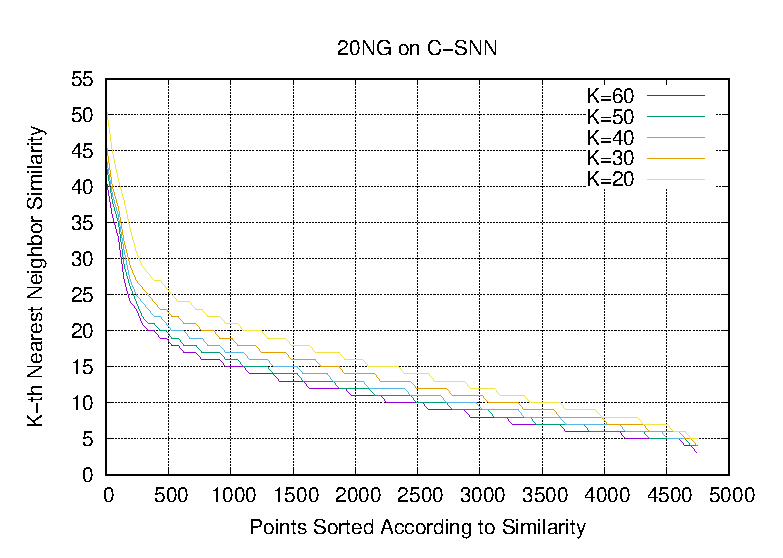
\includegraphics[width=\textwidth]{./tuning_figs/20NG_C-SNN.eps}
        %\caption{Tuning of 20NG on C-SNN.}
        \label{fig:20ng_tun_csnn}
    \end{subfigure}
    \begin{subfigure}[b]{0.37\textwidth}
        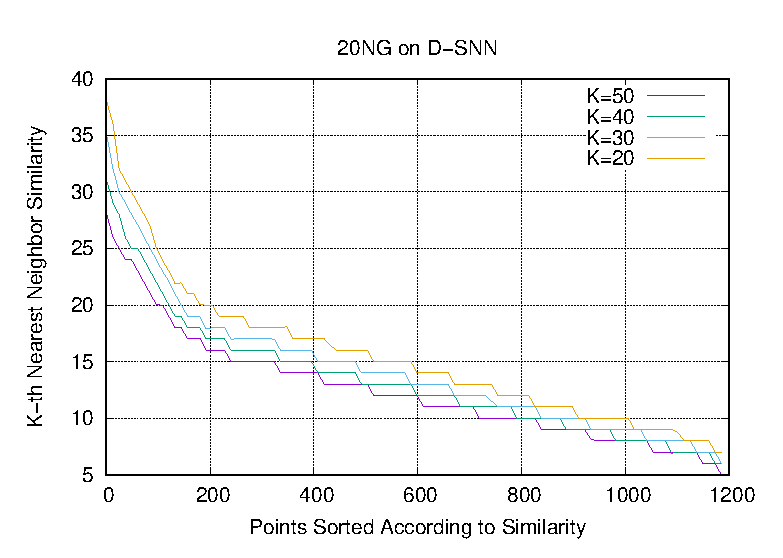
\includegraphics[width=\textwidth]{./tuning_figs/20NG_D-SNN.eps}
        %\caption{Tuning of 20NG on D-SNN.}
        \label{fig:20ng_tun_dsnn}
    \end{subfigure}
       \begin{subfigure}[b]{0.37\textwidth}
        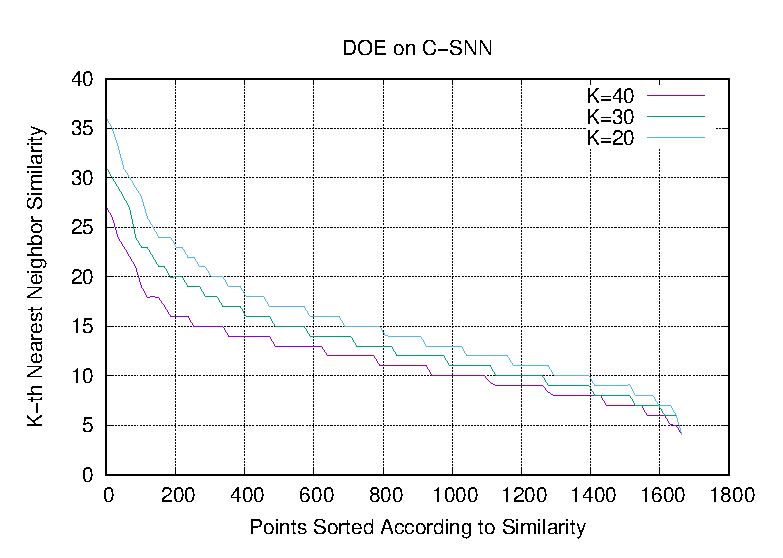
\includegraphics[width=\textwidth]{./tuning_figs/DOE_C-SNN.eps}
        %\caption{Tuning of 20NG on C-SNN.}
        \label{fig:doe_tun_csnn}
    \end{subfigure}
    \begin{subfigure}[b]{0.37\textwidth}
        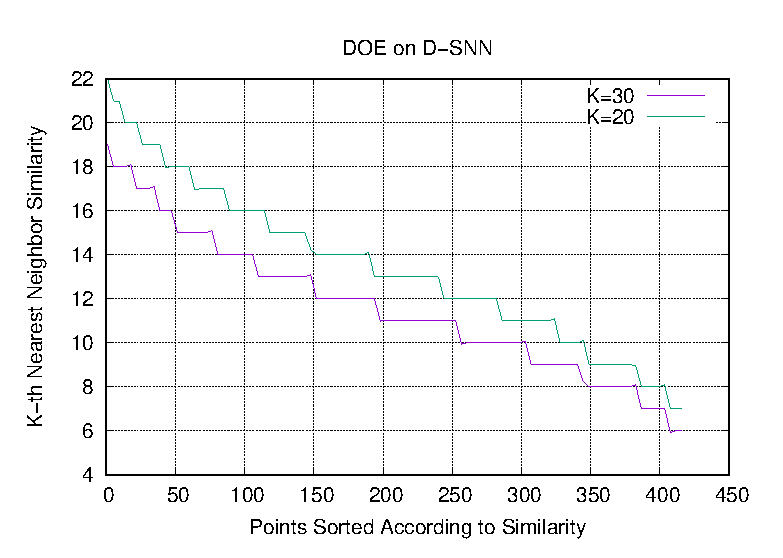
\includegraphics[width=\textwidth]{./tuning_figs/DOE_D-SNN.eps}
        %\caption{Tuning of 20NG on D-SNN.}
        \label{fig:doe_tun_dsnn}
    \end{subfigure}
    \begin{subfigure}[b]{0.37\textwidth}
        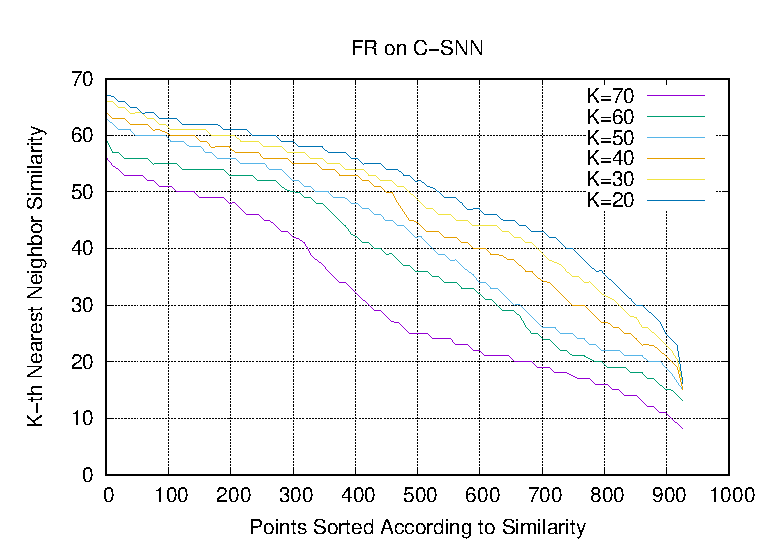
\includegraphics[width=\textwidth]{./tuning_figs/FR_C-SNN.eps}
        %\caption{Tuning of 20NG on C-SNN.}
        \label{fig:fr_tun_csnn}
    \end{subfigure}
    \begin{subfigure}[b]{0.37\textwidth}
        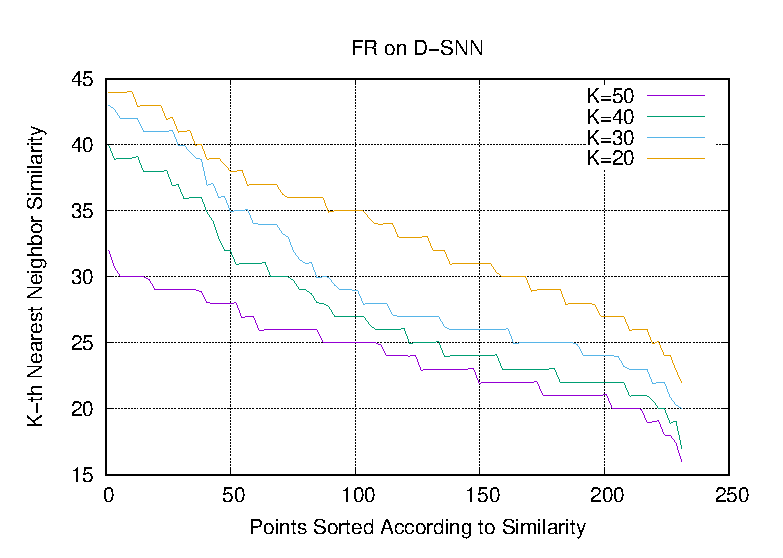
\includegraphics[width=\textwidth]{./tuning_figs/FR_D-SNN.eps}
        %\caption{Tuning of 20NG on D-SNN.}
        \label{fig:fr_tun_dsnn}
    \end{subfigure}
    \begin{subfigure}[b]{0.37\textwidth}
        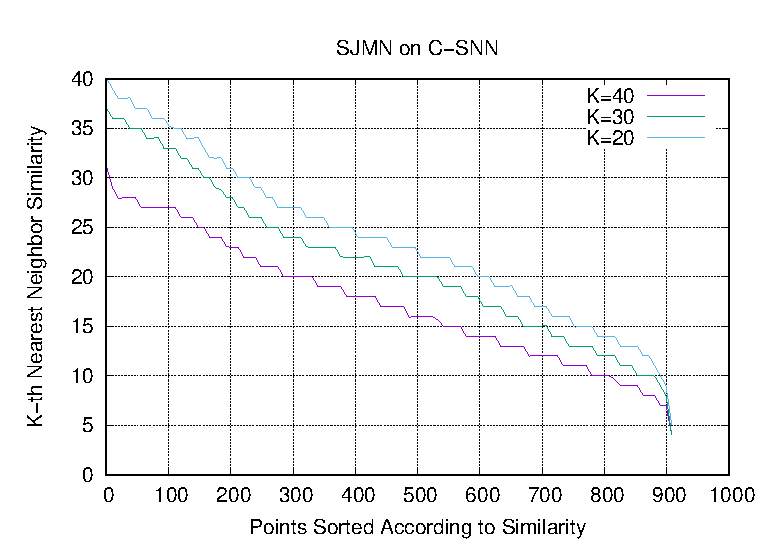
\includegraphics[width=\textwidth]{./tuning_figs/SJMN_C-SNN.eps}
        %\caption{Tuning of 20NG on C-SNN.}
        \label{fig:sjmn_tun_csnn}
    \end{subfigure}
    \begin{subfigure}[b]{0.37\textwidth}
        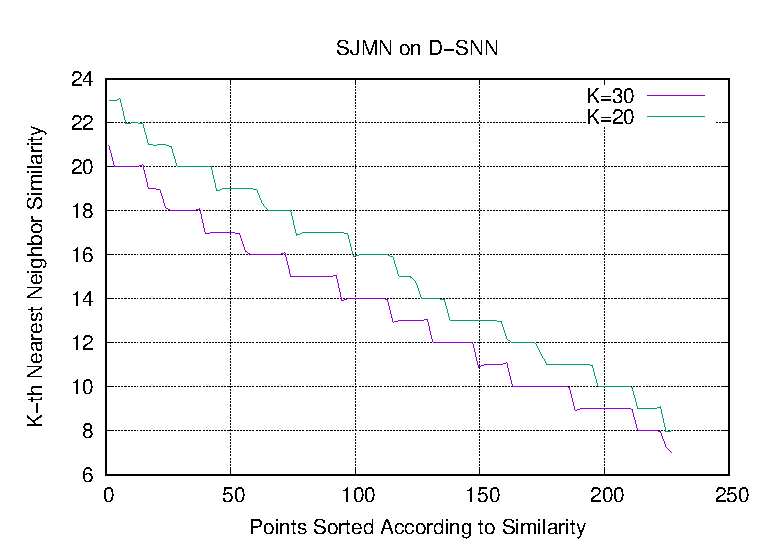
\includegraphics[width=\textwidth]{./tuning_figs/SJMN_D-SNN.eps}
        %\caption{Tuning of 20NG on D-SNN.}
        \label{fig:sjmn_tun_dsnn}
    \end{subfigure}
    \begin{subfigure}[b]{0.37\textwidth}
        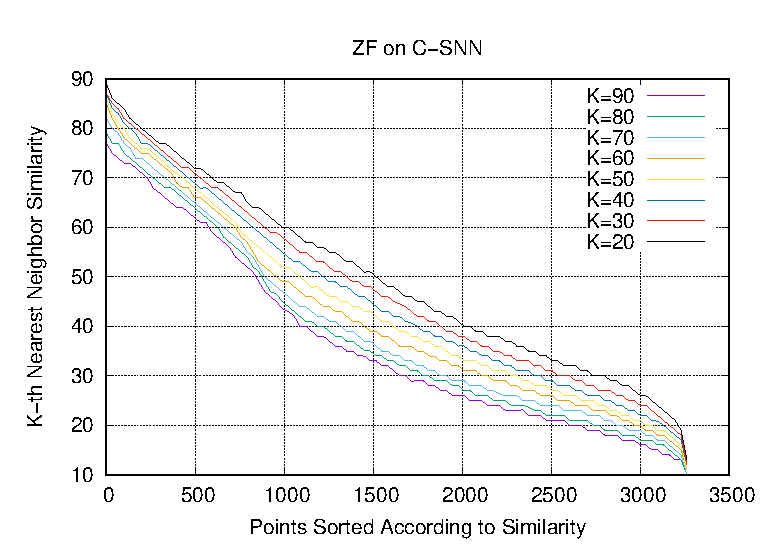
\includegraphics[width=\textwidth]{./tuning_figs/ZF_C-SNN.eps}
        %\caption{Tuning of 20NG on C-SNN.}
        \label{fig:zf_tun_csnn}
    \end{subfigure}
    \begin{subfigure}[b]{0.37\textwidth}
        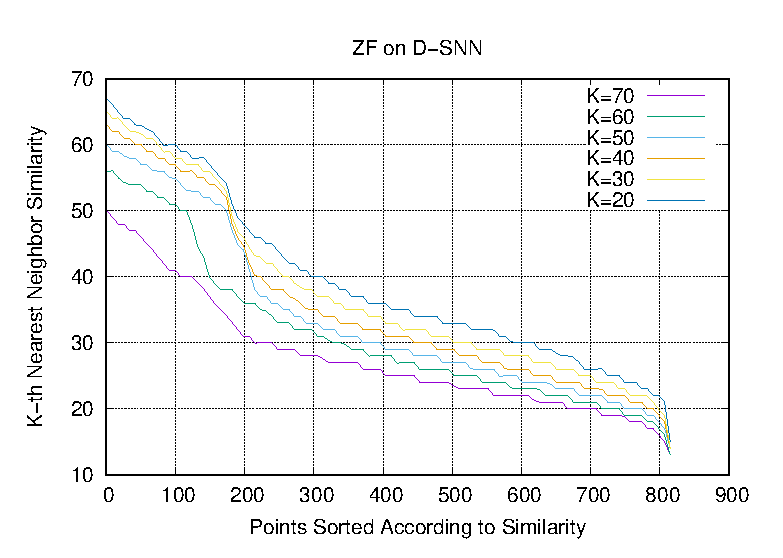
\includegraphics[width=\textwidth]{./tuning_figs/ZF_D-SNN.eps}
        %\caption{Tuning of 20NG on D-SNN.}
        \label{fig:zf_tun_dsnn}
    \end{subfigure}
    \caption{Tuning on C-SNN and D-SNN over the five data sets.}\label{fig:tun_curves}
\end{figure}

We noted that the shape of each plot is almost insensitive to $k$. Different values of $k$ produce a rescaling of the plot in terms of distances values but the shape remains the same.  
As sorted k-sim graphs are insensitive to $k$, we can fix $k$ following other criteria. On the one hand, an important criteria to fix $k$ is to avoid unnecessary computation. A high value of $k$ will demand the maintenance of large neighborhoods lists for SNN calculation. On the other hand, a low value of $k$ may discard close points in high density regions. We propose to use a value for $k$ estimating a fraction of the data set. The fraction is proportional to the density of the data set in the original space. The higher the density of the space, the higher the value of $k$. To avoid a linear increment on $K$ due to data size, we introduce a sublinear factor $\log(n_p)$, where $n_p$ corresponds to the size of the data partition. Note that for C-SNN, $n_p = n$. Then we estimate $k$ by:

\[ k = \frac{n}{100} \cdot \textsf{nnz} \cdot \log(n_p) . \]

For instance, in 20NG as $n=4743$, and $\mathsf{nnz} = 0.167$, then $k \approx 63$ for C-SNN and $52$ for D-SNN. Then we round $k$ to the closest number power of 5. 

Now to tune $\mathsf{MinPts}$, we produce sorted k-sim plots for several values of k. 
The highest value of k = $k$ (rounded), is useful to start the search of k from $k$ in decreasing order, in decrements of 10. These curves are shown in Figure \ref{fig:tun_curves}.

Low values of k produces less convex curves and high values of similarities. 
Ester \textit{et al.} \cite{E96} observed convex curves for k-sim graphs (DBSCAN was evaluated using k=4). 
We propose to use the sensitivity to k of sorted k-sim graphs to tune $\mathsf{MinPts}$ and $\mathsf{Eps}$. 

We tune $\mathsf{MinPts}$ to the lower value of k that produce a convexity in the k-sim plot. We conduct a search by descent for $\mathsf{MinPts}$, starting from $k$. A binary or galloping search on k is advisable to avoid unnecessary computation of k-sim curves when $k$ is high. Figure \ref{fig:tun_curves} shows the results of this procedure over the five data sets used in the previous section using both algorithms. In some cases, all the curves are almost equals in terms of convexity (e.g. see the curves for 20NG or SMNJ). In these cases, we choose the value that is in the middle of the search range. In other cases, the change in convexity is more notorious (e.g. see the curves for FR or ZF). Note that when $\mathsf{MinPts}$ is found, $\mathsf{Eps}$ is retrieved using the knee of the curve (the projection of the point to the y-axis). Figure \ref{fig:tun_curves} shows that the values found using our heuristic are similar to the ones showed using grid search with the exception of 20NG, where the value of $k$ was overestimated. The results of both algorithms using our tuning heuristic in terms of cluster quality are shown in Table \ref{table:tune}.

% table here!

\begin{table}[!htbp]
\centering
\begin{tabular}{|l|l|c|c|c|c|}
\hline
Data Set  &  Algorithm &  k  & $\mathsf{MinPts}$ & $\mathsf{Eps}$ & $\mathsf{VM}$ \\
\hline \hline
20NG      &  C-SNN     &  65 &  30  &  20  &  0.36  \\  
DOE       &  C-SNN     &  40 &  30  &  20  &  0.53  \\
FR        &  C-SNN     &  70 &  40  &  50  &  0.61  \\
SJMN      &  C-SNN     &  45 &  30  &  25  &  0.65  \\
ZF        &  C-SNN     &  95 &  60  &  60  &  0.44  \\
20NG      &  D-SNN     &  50 &  30  &  15  &  0.65  \\
DOE       &  D-SNN     &  35 &  20  &  10  &  0.79  \\
FR        &  D-SNN     &  35 &  20  &  25  &  0.69  \\
SJMN      &  D-SNN     &  35 &  30  &  15  &  0.67  \\
ZF        &  D-SNN     &  55 &  30  &  40  &  0.74  \\
\hline
\end{tabular}
\caption{Performance attained by C-SNN and D-SNN over the text collections using the tuning heuristic. Clustering quality results in terms of $\textsf{VM}$ are shown in the last column.}
\label{table:tune}
\end{table}

Table \ref{table:tune} shows the results in terms of $\mathsf{VM}$ after using our tuning procedure. This scenario is close to a real \textit{in production} scenario, where the clustering task is conducted over unlabeled data and accordingly the search for the optimum clustering solution is at some extent blind. We note that D-SNN outperforms C-SNN in all the comparisons, but paying the cost of a suboptimal parameter tuning that decreases the performance for both algorithms. These results show that C-SNN and D-SNN are sensitive to parameter tuning, and an inadequate setting may decrease the performance of D-SNN. Under this scenario, D-SNN exhibits a good performance. We understand that the use of partitions and the distributed nature of the algorithm are able to reduce the impact of parameter tuning on performance. In general, density-based clustering algorithms are very sensitive to parameter tuning. We evidence that a distributed density-based algorithm can limit the impact of a bad tuning, fact that aggregate an additional good property to our algorithm. 

\section{Conclusions and future work}
\label{sec:conc}

In this work, a distributed clustering method able to deal with massive text collections is proposed. In order to assess its utility especially for recovering the group structure underlying each collection, its performance is contrasted against two centralized approaches.
In addition, its performance was compared to k-means$||$, a fast implementation of the famous clustering algorithm in Spark. Our algorithm outperformed all these algorithms on five different data sets.  

Five real text collections were employed with the aim to show the weaknesses and strengths of the shared-nearest-neighbor approach in an isolated way from the strengths of the proposed method. The results indicate that D-SNN, besides its power to process big collections in a distributed fashion, maintains the good properties of C-SNN and at the same time improves the capability of dealing with the low discrimination power of the underlying similarity measure. 

%% OJO  CON ESTA FRASE ...
The proposed method can be easily extended to obtain a hypothetical labeling for each data point of the collection. That is, after the final stage in the central node, the labels of the clustered core-points can be re-transmitted to their original workers. Then, the local documents can be labeled according to their nearest core-point label.
Nevertheless although this task is very important for automatic tagging of collections (e.g. Automatic generation of Web directories), we think that the main contribution of this work lies in the \textit{cluster recovery task}, whose aim is to obtain a summary of the groups hidden in a large or a distributed collection unfeasible to process on a single machine. 

As future work we propose to provide an implementation of D-SNN on a big-data framework as Mahout and/or Spark. An big data implementation of D-SNN will able to test the scalability of our proposal, that, as was pointed out in this paper, has a low complexity in terms of computational costs. As our experiments show that D-SNN is very effective in terms of clustering quality, the addition of good scalability properties will provide at the same time a fast and effective distributed clustering algorithm for researchers and practitioners. 

\section{Acknowledgment}
H\'ector Allende-Cid was supported by project Fondecyt initiation into research 11150248.
Juan Zamora was supported by Fondecyt postdoc project 3180689.
Marcelo Mendoza was funded by Conicyt PIA/Basal FB0821.
\clearpage 

\bibliographystyle{apalike}
% \bibliography{references}
\begin{thebibliography}{}

\bibitem{BMVKV12}
Bahmani, B., Moseley, B., Vattani, A., Kumar, R., and Vassilvitskii, S. (2012).
\newblock {Scalable K-Means ++}.
\newblock {\em Proceedings of the VLDB Endowment (PVLDB)}, 5:622--633.

\bibitem{BEL13}
Balcan, M.~F., Ehrlich, S., and Liang, Y. (2013).
\newblock {Distributed k -Means and k -Median Clustering on General
  Topologies}.
\newblock {\em Advances in Neural Information Processing Systems 26 (NIPS
  2013)}, pages 1--9.

\bibitem{CM13}
Crestani, F., and Markov, I. (2013).
\newblock {Distributed Information Retrieval and Applications}.
\newblock {\em 35th European Conference on IR Research}, 865--868.

\bibitem{DDGR07}
Das, A., Datar, M., Garg, A., and Rajaram, S. (2007).
\newblock Google news personalization: scalable online collaborative filtering.
\newblock In {\em Proceedings of the 16th international conference on World
  Wide Web}, pages 271--280. ACM.

\bibitem{VVGN15}
De~Vries, C.~M., De~Vine, L., Geva, S., and Nayak, R. (2015).
\newblock Parallel streaming signature {EM}-tree: A clustering algorithm for web
  scale applications.
\newblock In {\em Proceedings of the 24th International Conference on World
  Wide Web}, pages 216--226. ACM.

\bibitem{DM99}
Dhillon, I.~S. and Modha, D.~S. (1999).
\newblock {A data-clustering algorithm on distributed memory multiprocessors}.
\newblock {\em Large-Scale Parallel Data Mining}, 1759(802):245--260.

\bibitem{EIM11}
Ene, A., Im, S., and Moseley, B. (2011).
\newblock {Fast Clustering using MapReduce}.
\newblock {\em Kdd}, 681--689.

\bibitem{E96}
Ester, M., Kriegel, H., Sander, J. and Xu X. (1996). 
\newblock {A density-based algorithm for discovering clusters}.
\newblock In {\em Proceedings of the 2nd International Conference on Knowledge Discovery and Data Mining}, pages 226--211.

\bibitem{ESK03}
Ert{\"o}z, L., Steinbach, M., and Kumar, V. (2003).
\newblock {Finding clusters of different sizes, shapes, and densities in noisy, high dimensional data}.
\newblock {\em Proceedings of the SIAM International Conference on Data Mining}, 47--58.

% \bibitem[Ester et~al., 1996]{EKSX96}
% Ester, M., Kriegel, H., Sander, J., and Xu, X. (1996)
% \newblock {A density-based algorithm for discovering clusters in large spatial databases with noise}.
% \newblock {\em Proceedings of the Second International Conference on Knowledge Discovery and Data Mining}, 96:226--231.

\bibitem{FZ00}
Forman, G. and Zhang, B. (2000).
\newblock {Distributed data clustering can be efficient and exact}.
\newblock {\em ACM SIGKDD Explorations Newsletter}, 2(2):34--38.

\bibitem{GRS98}
Guha, S., Rastogi, R. and Shim, K. (1998).
\newblock{CURE: an efficient clustering algorithm for large databases}.
\newblock{\em ACM SIGMOD Record},  27(2):73--84.

%\bibitem{HK11}
%Han, J., Pei, J., and Kamber, M. (2011).
%\newblock {\em Data mining: concepts and techniques}.
%\newblock Elsevier.

%\bibitem{I14}
%Indra, Z., Zamin, N., Jaafar, J. (2014).
%\newblock{A clustering technique using single pass clustering algorithm for search engine}.
%\newblock{\em 2014 4th World Congress on Information and Communication Technologies (WICT 2014)},  1:182--187.

\bibitem{Tal02}
Talia, D. (2002)
\newblock{Parallelism in Knowledge Discovery Techniques}
\newblock{In PARA '02: Proceedings of the 6th International Conference on Applied Parallel Computing Advanced Scientific Computing, pages 127-138, London, UK, 2002. Springer-Verlag. }

\bibitem{JW05}
Jagannathan, G., and Wright, R. N. (2005).
\newblock {Privacy-preserving Distributed K-means Clustering over Arbitrarily Partitioned Data}.
\newblock {\em Proceedings of the Eleventh ACM SIGKDD International Conference on Knowledge Discovery in Data Mining}, 593--599.

%\bibitem{JKP03}
%Januzaj, E., Kriegel, H.-P., and Pfeifle, M. (2003).
%\newblock {Towards Effective and Efficient Distributed Clustering}.
%\newblock {\em Workshop on Clustering Large Data Sets}, pages 49--58.

\bibitem{JKP04}
Januzaj, E., Kriegel, H.-P., and Pfeifle, M. (2004).
\newblock {Scalable Density-Based Distributed Clustering}.
\newblock pages 231--244.

%\bibitem{JCHAC15}
%Jin, C., Chen, Z., Hendrix, W., Agrawal, A., and Choudhary, A. (2015).
%\newblock {Incremental, Distributed Single-linkage Hierarchical Clustering
%  Algorithm Using Mapreduce}.
%\newblock {\em Proceedings of the Symposium on High Performance Computing},
%  pages 83--92.

%\bibitem{JK00}
%Johnson, E. and Kargupta, H. (2000).
%\newblock {Collective, hierarchical clustering from distributed, heterogeneous
%  data}.
%\newblock {\em Lecture Notes in Computer Science}, 1759:221--244.

\bibitem{KHSJ01}
Kargupta, H., Huang, W., Sivakumar, K., and Johnson, E. (2001).
\newblock Distributed clustering using collective principal component analysis.
\newblock {\em Knowledge and Information Systems}, 3(4):422--448.

\bibitem{KLM03}
Klusch, M., Lodi, S., and Moro, G. (2003).
\newblock {Distributed clustering based on sampling local density estimates}.
\newblock {\em IJCAI International Joint Conference on Artificial
  Intelligence}, pages 485--490.

\bibitem{KKPS05}
Kriegel, H.-p., Kr, P., Pryakhin, A., and Schubert, M. (2005).
\newblock {Effective and Efficient Distributed Model-based Clustering}.

\bibitem{LZO03}
Li, T., Zhu, S., and Ogihara, M. (2003).
\newblock {Algorithms for Clustering High Dimensional and Distributed Data}.
\newblock {\em Intelligent Data Analysis Journal}, 7(February):1--36.

\bibitem{LBK13}
Liang, Y., Balcan, M.-f., and Kanchanapally, V. (2013).
\newblock {Distributed PCA and k-Means Clustering}.
\newblock {\em The Big Learning Workshop in NIPS 2013}, pages 1--8.

\bibitem{LHLX12}
Liu, J., Huang, J. Z., Luo, J., and Xiong, L. (2012).
\newblock {Privacy Preserving Distributed DBSCAN Clustering}.
\newblock {\em Proceedings of the 2012 Joint EDBT/ICDT Workshops}, 177--185.

\bibitem{Mendoza16}
Mendoza, M., Mar\'in, M., Gil-Costa, V., and Ferrarotti, F. (2016). 
\newblock {Reducing hardware hit by queries in web search engines}.
\newblock {\em Information Processing \& Management}, 52(6):1031 - 1052.

\bibitem{MG03}
Merugu, S. and Ghosh, J. (2003).
\newblock {Privacy-preserving Distributed Clustering using Generative Models}.
\newblock {\em Proceedings of the 3rd IEEE International Conference on Data
  Mining (ICDM)}, pages 0--7.

\bibitem{N15}
Nagwani, N. K. (2015).
\newblock {Summarizing large text collection using topic modeling and clustering based on MapReduce framework}.
\newblock {\em Journal of Big Data}, 2:1--18.

%\bibitem{NC14}
%Naldi, M.~C. and Campello, R. J. G.~B. (2014).
%\newblock {Evolutionary k-means for distributed data sets}.
%\newblock {\em Neurocomputing}, 127:30--42.

%\bibitem{ZLW08}
%Qi, Z., Jinze, L., and Wei, W. (2008).
%\newblock {Approximate clustering on distributed data streams}.
%\newblock {\em Proceedings - International Conference on Data Engineering},
%  00:1131--1139.

%\bibitem{R87}
%Rousseeuw Peter J. (1987). 
%\newblock {Silhouettes: A graphical aid to the interpretation and validation of cluster analysis}.
%\newblock {\em Journal of Computational and Applied Mathematics}, 20:53--65.

\bibitem{SC16}
Sarnovsky, M., Carnoka, N.. (2016). 
\newblock {Distributed Algorithm for Text Documents Clustering Based on k-Means Approach}.
\newblock {\em Advances in Intelligent Systems and Computing}, 430:165--174.

\bibitem{VEB10}
Vinh, Nguyen X. and Epps, J. and Bailey, J. (2010).
\newblock{Information theoretic measures for clustering comparison: Variants, properties, normalization and correction for chance}.
\newblock{\em Journal of Machine Learning Research}, 11:2837--2854.

\bibitem{Vis08}
Visalakshi, N.K., Thangavel, K., Alagambigai, P. (2008)
\newblock{Distributed Clustering for Data Sources with Diverse Schema}
\newblock{International Conference on Convergence and Hybrid Information Technology, Busan South Korea, 2008, 1056-1061.}

\bibitem{XJK99}
Xu, X., J{\"{a}}ger, J. and Kriegel, H. (1999).
\newblock {A fast parallel clustering algorithm for large spatial databases}.
\newblock {\em High Performance Data Mining}, 290:263--290.

\bibitem{Yi14}
Yi, J., ZShang, L., Wang, J., Jin, R., Jain, A.K. (2014)
\newblock {A Single-Pass Algorithm for Efficiently Recovering Sparse Cluster Centers of High-dimensional Data}.
\newblock {\em Proceedings of the 31 st International Conference on Machine
Learning, Beijing, China, 2014.}, 3:2112--2127.

\bibitem{ZW13}
Zhang, J., Wu, G., Hu, X., Li, S., Hao, S. (2013).
\newblock{A Parallel Clustering Algorithm with MPI – MKmeans }.
\newblock{\em Jouirnal of Computers}, 8(1):10--18.

\bibitem{ZK02}
Zhao, Y. and Karypis, G. (2002).
\newblock{Evaluation of hierarchical clustering algorithms for document datasets}.
\newblock{\em Proceedings of the eleventh international conference on Information and knowledge management}, 515--524.

\end{thebibliography}
\end{document}